\chapter{n-3 Polyunsaturated Fatty Acid Rich Diet in Schizophrenia}
\label{omegaProject}
\section{Introduction}
\glsreset{mia}
\glsreset{pufa}
\glsreset{polyic}
\glsreset{gd}
In the previous chapter, we have found that the \gls{SNP} heritability of \glng{scz} is estimated to be at most 20\% which is much lower than expected in \glng{scz}.
This suggests that other factors such as rare variants such, epigenetic factors and gene-environmental interaction ($G\times E$) might contribute to the ``missing'' heritability of \glng{scz}.

Previous studies have reported the possibility of interaction between prenatal infection and genetic variation in risk of developing \glng{scz} \citep{Tienari2004,Clarke2009}.
It has been suggested that the effect of prenatal infection was mainly mediated by maternal immune response, instead of the specific type of infection \citep{Brown2010}.
Therefore it is likely for the perturbation induced by \gls{mia} to interact with genetic variations in the development of \glng{scz}.

Slowly but steadily, progress has been made in the research of \glng{scz}.
Converging evidence from \gls{GWAS}, \gls{cnv} and sequencing studies suggest that rare and common variants in genes related to \gls{psd} \citep{Purcell2014,Consortium2015a} and calcium ion channels \citep{Purcell2014,Ripke2014,Szatkiewicz2014} contribute to the etiology of \glng{scz}.
Given these, it is possible for the effect of prenatal infection to also act upon the same functional gene sets during the development of \glng{scz}.

Additionally, with the development of \gls{ldsc}, partitioning of \gls{SNP} heritability can now be performed using summary statistics from \gls{GWAS}. 
It is therefore possible to not only identify gene sets or pathways that are associated with \glng{scz}, but also estimate their relative contribution to the heritability of \glng{scz}.

Furthermore, a number of studies have reported the potential of n-3 \gls{pufa} in the treatment of \glng{scz} \citep{Li2015,Trebble2003}. 
In mouse, it was found that n-3 \gls{pufa} can inhibits the production of \gls{il6} \citep{Trebble2003} - a major mediator in \gls{mia} model \citep{Smith2007}.
Apart from its anti-inflammatory property, n-3 \gls{pufa} such as docosahexaenoic acid (DHA) also plays a critical role in the development of central nervous system \citep{Clandinin1999,Kitajka2002}.
Given its strong implication in neuronal functioning, it is possible that n-3 \gls{pufa} rich diet may reduce the symptoms of \glng{scz}, as reported by a recent study \citep{Li2015}.

% Cerebellum
Herein, we conduct a hypothesis-driven study to investigate the gene expression changes induced by early \gls{mia} exposure in the brain of the adult offspring, and also expression changes induced by n-3 \gls{pufa} rich diet using RNA Sequencing.
Another goal of the current study is to investigate whether the effects of \gls{mia} or diet act upon the same functional gene sets as the genetic variants associated with \glng{scz} in the development of the disease.
Finally, the relative contribution of the candidate gene sets to the heritability of \glng{scz} was also estimated using \gls{ldsc}.

Although hippocampus \citep{Velakoulis2006,Nugent2007} and prefrontal cortex \citep{Knable1997,Perlstein2001} are the two brain regions that have been extensively studied in \glng{scz}, cerebellum dysfunction has also been reported in \glng{scz} \citep{Yeganeh-Doost2011,Andreasen2008}.
Specifically, \gls{pet} studies have shown that a dysfunction in the cortico-cerebellar-thalamic-cortical neuronal circuit, which contributes to ``cognitive dysmetria'', e.g. impaired cognition, and other symptoms of \glng{scz} \citep{Yeganeh-Doost2011}.
Taken together, cerebellum might plays an important part in the etiology of \glng{scz} and are therefore selected for the current study. 

The work in this chapter were done in collaboration with my colleagues who have kindly provide their support and knowledges to make this piece of work possible.
Dr Li Qi and Dr Basil Paul were responsible for generating the animal model and providing the sample for our study;
Dr Li Qi and Dr Desmond Campbell helped with the experimental design;
Vicki Lin has helped with the RNA extraction; 
Tikky Leung for her high quality sequencing service;
Nick Lin for his help in tackling problems encountered during sequencing quality control; 
Dr Johnny Kwan, Dr Desmond Campbell, Dr Timothy Mak and Professor Sham for their guidance in the statistical analysis.

\section{Methodology}
\subsection{Sample Preparation}
Female and male C57BL6/N mice were bred and mated by The University of Hong Kong, Laboratory Animal Unit. 
Timed-pregnant mice were held in a normal light–dark cycle (light on at 0700 hours), and temperature and humidity-controlled animal vivarium. 
All animal procedures were approved by the Committee on the Use of Live Animals in Teaching and Research (CULATR) at The University of Hong Kong.

The \gls{mia} model was generated following procedures previously reported \citep{Li2009c}. 
A dose of 5mg kg$^{-1}$ \gls{polyic} in an injection volume 5ml kg$^{-1}$, prepared on the day of injection was administered to pregnant mice on \gls{gd} 9 via the tail vein under mild physical constraint. 
Control animals received an injection of 5ml kg$^{-1}$ 0.9\% saline. 
The animals were returned to the home cage after the injection and were not disturbed, except for weekly cage cleaning.
The resulting offspring were weaned and sexed at postnatal day 21. 
The pups were weighed and littermates of the same sex were caged separately, with three to four animal per cage.
Half of the animal were fed on diets enriched with n-3 \glspl{pufa} and half were fed a standard  lab diet until the end of the study.
The latter `n-6 \gls{pufa}' control diet had the same calorific value and total fat content as the n-3 \gls{pufa} diet. 
The diets were custom prepared and supplied by Harlan Laboratories (Madison, WI, USA). 
The n-6 and n-3 \gls{pufa} were derived from corn oil or menhaden fish oil, respectively. 
The n-6 \gls{pufa} control diet, was based on the standard AIN-93G rodent laboratory diet \citep{Reeves1993}, and contained 65 g kg$^{-1}$ corn oil and 5 g kg$^{-1}$ fish oil with an approximate (n6)/(n3) ratio of 13:1. 
The n-3 \gls{pufa} diet contained 35 g kg$^{-1}$ corn oil and 35 g kg$^{-1}$ fish oil with an approximate (n6)/(n3) ratio of 1:1 \citep{Olivo2005}.
To avoid being confounded by sex difference, we only use the male offspring for our analysis.
The male offspring were sacrificed by cervical dislocation on postnatal week 12, which roughly correspond to adulthood in human, and the cerebellum was extracted and stored in -80$^{\circ}$C until RNA extraction.

\subsection{RNA Extraction, Quality Control and Sequencing}
Total RNA was extracted from each cerebellum tissue using RNeasy midi kit (Qiagen) following the manufacturer's instructions.
RNA quality was assayed using the Agilent 2100 Bioanalyzer and RNA was quantified using Qubit 1.0 Flurometer.
Samples with \gls{rin} $<7$ were not included in our study as the RNA are most likely degraded.
As a hypothesis generation study, we select a minimum of 3 samples per group and each samples must come from a different litter to control for littering effect.
The RNA Sequencing library was performed at the Centre for Genomic Sciences, the University of Hong Kong, using the KAPA Stranded mRNA-Seq Kit. 
All samples were sequenced using Illumina HiSeq 1500 at 2 lanes (2$\times$101 \gls{bp} paired end reads).
We distribute the samples such that each lane contain roughly the same amount of samples from different conditions.
\begin{table}
	\centering
	\begin{tabular}{rrrrrrr}
		\toprule
		SampleID & Litter & Diet & Condition & Lane & Batch & Rin\\
		\midrule
		B1&	3&	O3&	POL&	1&	B&	7.7\\
		B2&	6&	O3&	POL&	2&	B&	7.7\\
		F1&	4&	O3&	POL&	1&	F&	7.6\\
		F4&	1&	O3&	SAL&	2&	F&	8.1\\
		B4&	5&	O3&	SAL&	1&	B&	7.8\\
		B5&	14&	O3&	SAL&	2&	B&	7.7\\
		F2&	2&	O6&	POL&	1&	F&	7.5\\
		E3&	11&	O6&	POL&	2&	E&	7.8\\
		C2&	7&	O6&	POL&	2&	C&	7.9\\
		B6&	13&	O6&	SAL&	2&	B&	7.4\\
		E6&	14&	O6&	SAL&	1&	E&	8\\
		C6&	1&	O6&	SAL&	1&	C&	7.8\\
		\bottomrule
	\end{tabular}
	\caption[Sample Information]{
		Sample information.
		O3 = n-3 \gls{pufa} diet; O6 = n-6 \gls{pufa} diet; POL = \gls{polyic} exposed; SAL = Saline exposed.
		We have tried to separate the samples into different lane and batch to control for the lane and batch effect. 
		Samples from different litters were also used with the exception of F4 and C6 which came from the same litter but were given a different diet.
		\label{tab:sampleInfo}
	}
\end{table}
\subsection{Sequencing Quality Control}
\Gls{qc} of the RNA Sequencing read data was assessed by FastQC \citep{Andrews2010}, which reports the overall quality of the high throughput sequence, and allow the identification of any potential problems and biases.

From the FastQC report, it was noted that some adapter sequences remained in the final sequence.
By using trim\_glore, a wrapper for cutadapt (version 1.9.1) \citep{Martin2011}, the adapter sequences were removed from the sequence reads and only reads that were at least 75 \gls{bp} long were retained for subsequent alignment. 

\subsection{Alignment}
In a recent review by \citet{Engstrom2013}, it was demonstrated that STAR \citep{Dobin2013} has the best performance in term of accuracy and speed among all the aligners investigated.
Thus STAR aligner was used in our study.
The RNA sequencing reads were mapped to the \textit{Mus musculus} reference genome (mm10, Ensembl GRCm38.82) using the STAR aligner (version 2.5.0a) \citep{Dobin2013}.
And the quantification of the gene expression levels were conducted using featureCounts (version 1.5.0) \citep{Liao2014}.

\subsection{Data Quality Assessment}
Data quality assessment and quality control are essential steps of any data analysis. 
In order to assess the quality of the count data, unsupervised clustering was performed.
Sample with abnormal count data was removed from the analysis. 

\subsection{Differential Expression Analysis}
There are many statistical tools available for the differential gene expression analysis.
Based on the review of \citet{Seyednasrollah2015}, it was suggested that DESeq2 and limma are the most robust statistical packages for analyzing RNA Sequencing data. 
As the authors of DESeq2 are very active in providing supports for the package, DESeq2 (version 2.1.4.5) \citep{Love2014} was used as the statistic package for the differential gene expression analysis.

One of the most controversial RNA sequencing study  in RNA Sequencing was the mouse ENCODE study by \citet{Yue2014}, where most of the findings reported were found to be confounded by lane and batch effect \citet{Gilad2015}.
This highlights the importance of lane and batch effect in the design of RNA Sequencing.
To avoid batch and lane effect, the whole sampling collection procedure and sequencing was performed in a way where we minimize the batch and lane difference between conditions (\cref{tab:sampleInfo}). 
However, because of the sample quality differed across different batches, we were unable to fully balance out the batch effect. 
Therefore, it was necessary to control for batch effect in the analyzes.

The following statistical comparisons were performed:
\begin{enumerate}
	\item Saline exposed samples with n-3 \gls{pufa} rich diet vs Saline exposed samples with n-6 \gls{pufa} rich diet 
	\item PolyI:C exposed samples with n-3 \gls{pufa} rich diet vs PolyI:C exposed samples with n-6 \gls{pufa} rich diet 
	\item Saline exposed samples with n-6 \gls{pufa} rich diet vs PolyI:C exposed samples with n-6 \gls{pufa} rich diet 
\end{enumerate}
We used $\sim Batch+Condition+Diet+Condition:Diet$ as our model of statistical analysis where Condition is the \gls{mia} exposure status.
\Gls{rin} was not included in the statistical model as suggested by the author.
%
%To further investigate whether batch effect may can lead to false positives, we performed the \gls{lrt} to investigate the effect of batch on our result.
%The \gls{lrt} examines two models for the counts, a full model with a certain number of terms and a reduced model, in which some of the terms of the full model are removed. 
%The test determines if the increased likelihood of the data using the extra terms in the full model is more than expected if those extra terms are truly zero.
%Thus we compared the full model $\sim Batch+Condition+Diet+Condition:Diet$ with $\sim Condition+Diet+Condition:Diet$ to understand the effect of batch on our data.

In our analysis, genes with base mean count $<$ 10 were removed to reduce noise associated with low expression and the Benjamini and Hochberg method was then used to correct for multiple testing.

\subsection{Gene Set Analysis}
\label{sec:function}
The main goal of the current study is to investigate whether the effect of MIA or diet act upon the same functional gene sets as the genetic variants associated with schizophrenia in the development of the disease. 
Specifically, as genes related to \gls{psd} \citep{Purcell2014,Consortium2015a} and calcium ion channel \citep{Purcell2014,Ripke2014,Szatkiewicz2014} has been implicated to be involved in the etiology of \glng{scz}, it is interesting to investigate whether these gene sets were also enriched by genes perturbed by \gls{mia} or diet.

To compile a list of relevant gene-sets, significant gene sets from \citet{Purcell2014,Consortium2015a} were retrieved, which include gene set related to calcium ion channel and \gls{psd}.
Gene sets and pathway related to \gls{psd} and calcium ion channel were also retrieved from \gls{kegg} \citep{Kanehisa2000} and \gls{go} \citep{Consortium2015b}, both have been widely used for systematic genetic analysis.
In addition, the \glng{scz} \gls{GWAS} gene set, constructed based on associated \gls{GWAS} \gls{LD}-intervals from \citet{Ripke2013} by \citet{Purcell2014} was also included.


The Wilcoxon Rank Sum test was performed to assess whether the gene sets were enriched by genes affected by either \gls{mia} or diet.
Pathways with adjusted p-value $<0.05$ (using Benjamini and Hochberg adjustment) were considered as significant.

\subsection{Partitioning of Heritability}
In order to identify the relative contribution of the significant gene sets to the heritability of \glng{scz}, partitioning of heritability of \glng{scz} was performed using \gls{ldsc}.

Firstly, \glspl{SNP} were assigned to genes based on human genome hg19 positions if they lay within 35 \gls{kb} upstream or 10 \gls{kb} downstream of the gene.
If \glspl{SNP} mapped within more than one gene, they were assigned to all such genes, following the procedure employed by \citet{Consortium2015a}

Then, the partitioning of heritability was performed using \gls{ldsc} \citep{Bulik-Sullivan2015} -{}-annot and -{}-overlap-annot options, with window size of 1000\gls{kb} window size and the \gls{LD} score generated in \cref{sec:realData}.
The \gls{mhc} region (chr6:25,000,000-35,000,000) was removed from the analysis due to its unusual \gls{LD} and genetic architecture \citep{Finucane2015}.

\subsection{Designing the Replication Study}
The sample size of the current study is relatively small and therefore only serves as a pilot study.
It is therefore important to utilize the information from the current study to design a more powerful follow-up study.

In order to estimate the required sample size for the follow-up studies, power estimation was performed using Scotty \citep{Busby2013}.
Based on the current count data, Scotty can estimate the required sample size of the follow up study in order to detect at least 90\% of the differentially expressed genes with least 2$\times$ difference, and for at least 80\% of genes to reach 80\% of the maximum power.

\section{Results} 
\subsection{Sample Quality}
On average, 87 million reads were generated for each sample of which more than 90\% of the read bases has quality score $>30$.
More than 97\% of the sequence reads remains after adapter trimming was performed. 
Over 90\% of the trimmed reads were uniquely mapped to the \textit{Mus musculus} reference genome (mm10, Ensembl GRCm38.82) using the STAR aligner (version 2.5.0a) \citep{Dobin2013}.

Unsupervised clustering was performed to assess the count data quality. 
It is observed that none of the samples are clustered by lane or by batch (\cref{fig:distMatrix}).
However, one of the sample in the n3-\gls{polyic} group is found to be substantially different from all other samples. 
It is unclear whether the difference was a result of sample contamination from other sources, or was a result of sample mis-label.
The sample was therefore excluded from subsequent analyses.
 \begin{figure}
	\centering
	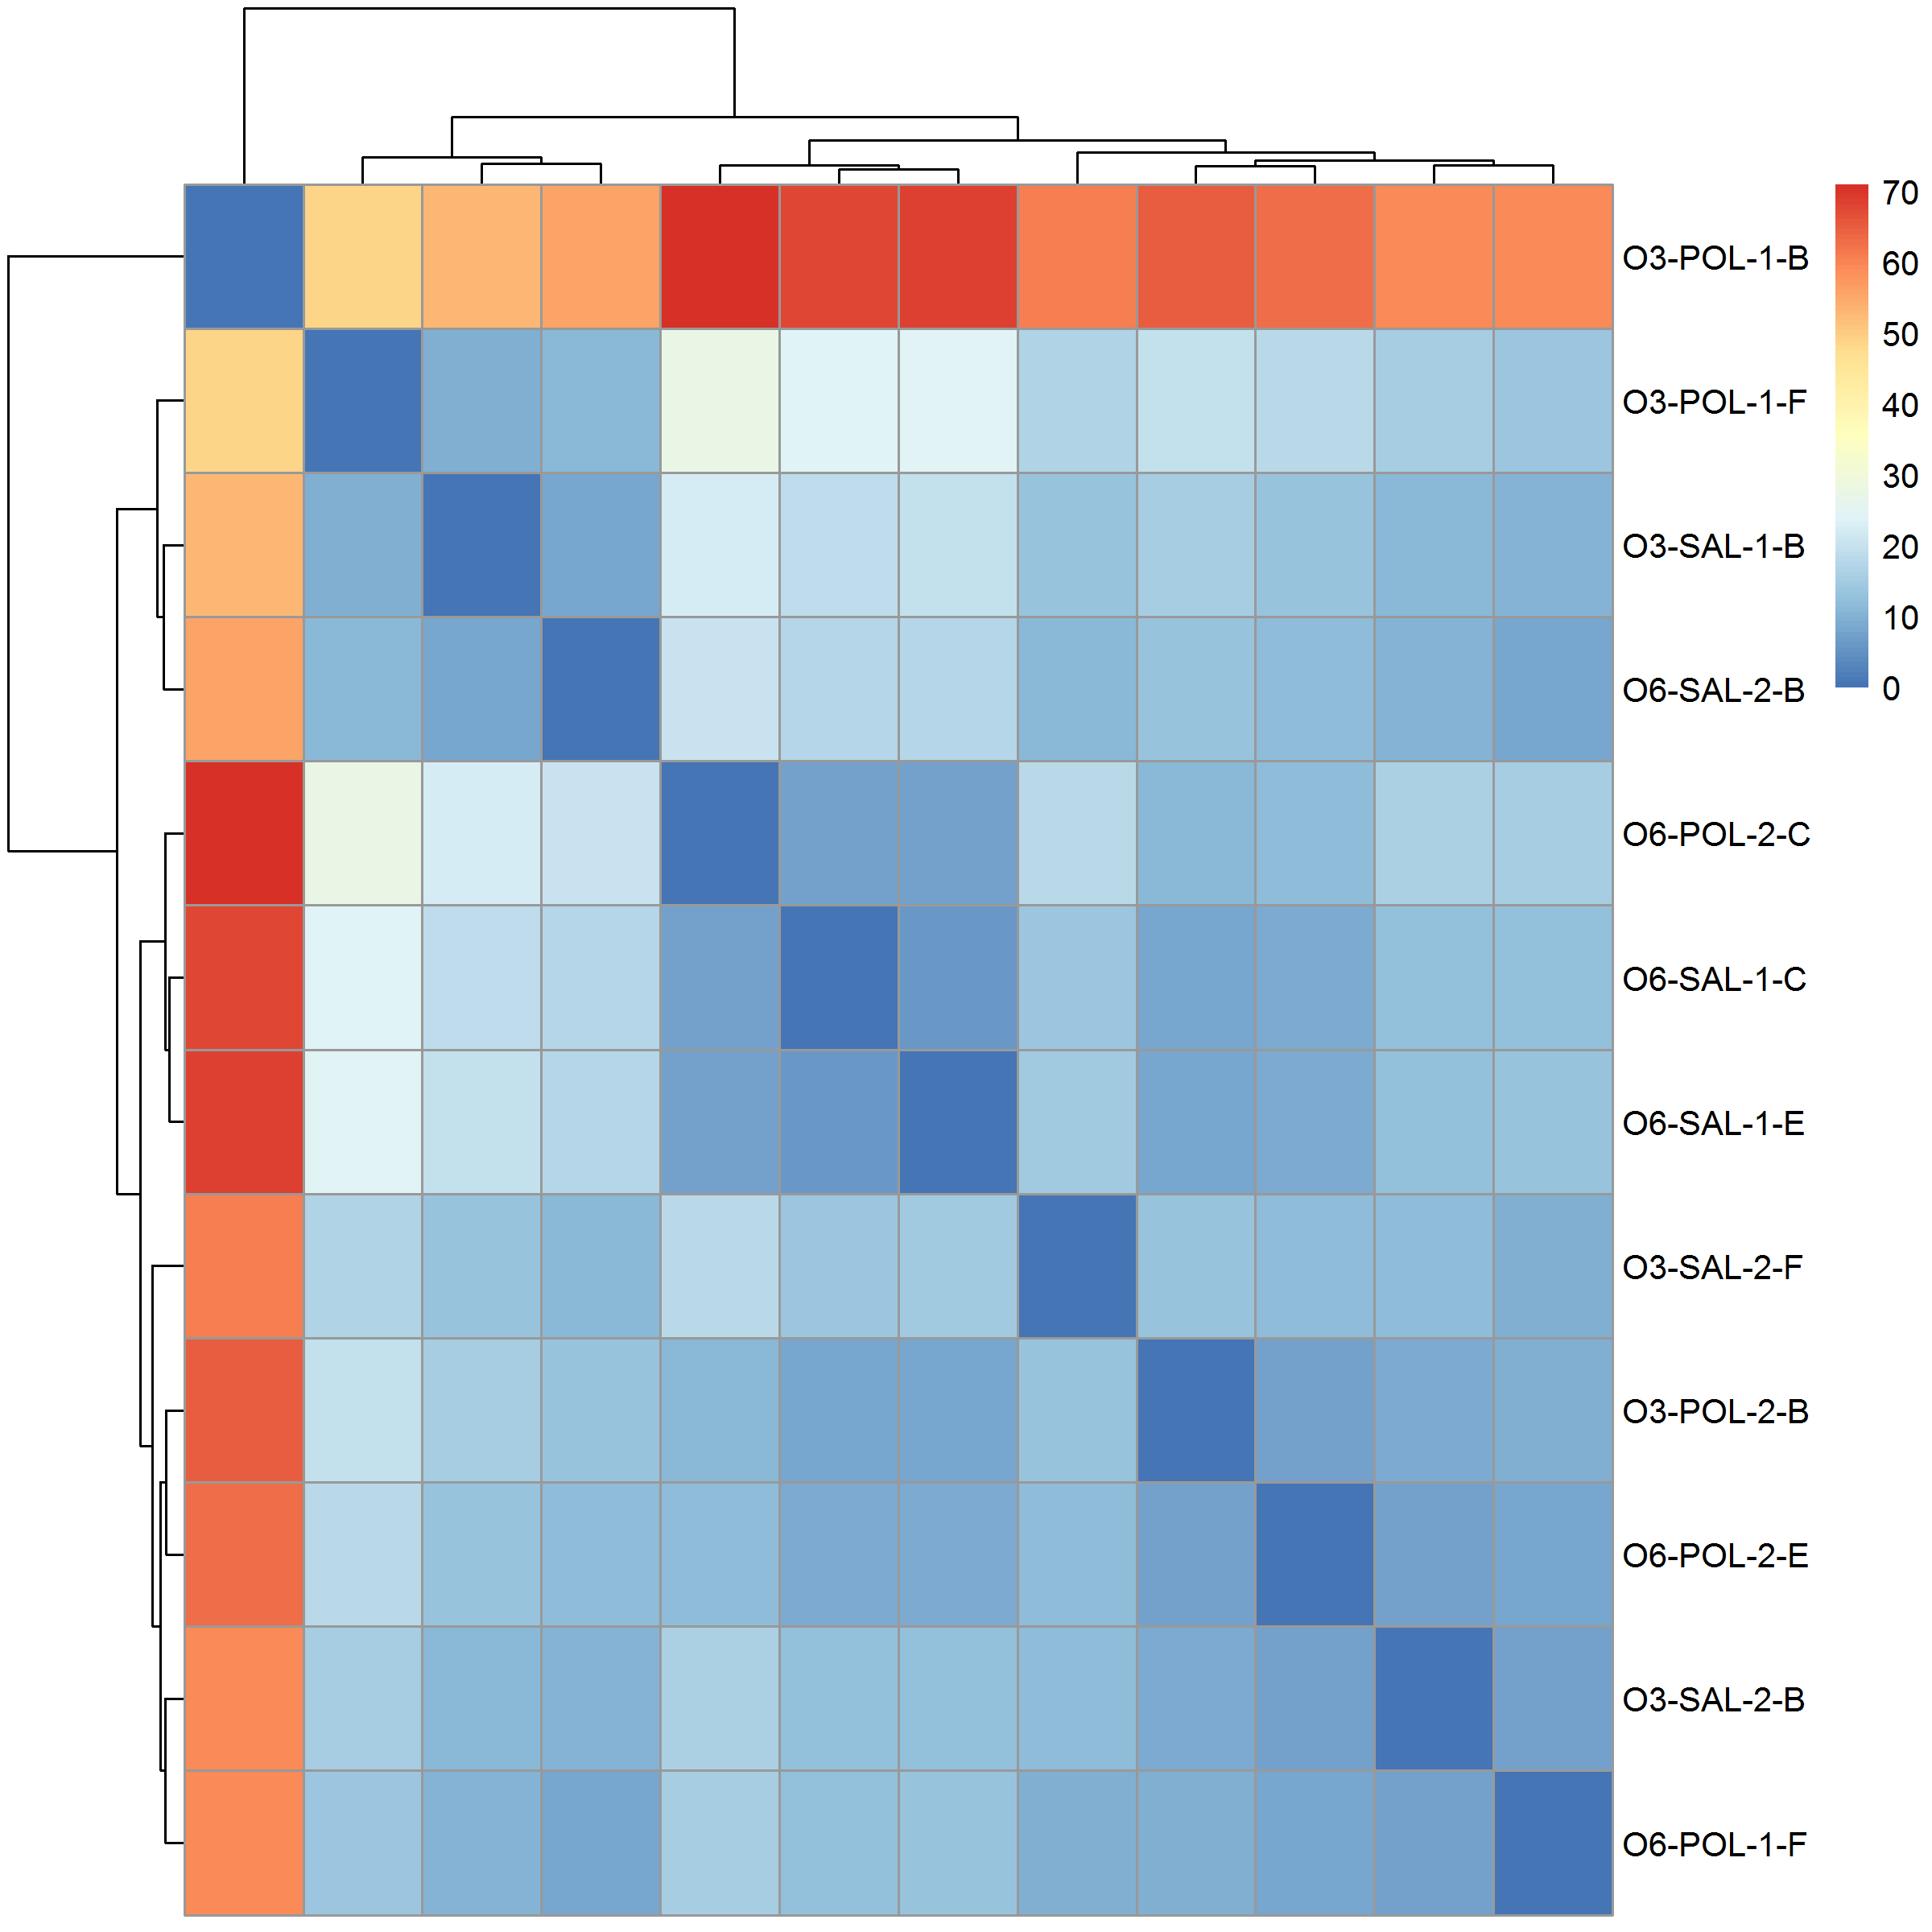
\includegraphics[width=0.7\textwidth]{figure/DistanceMatrix.png}
	\caption[Sample Clustering]{Sample Clustering results.
		Samples were labeled as $<$Diet$>$-$<$Condition$>$-$<$Lane$>$-$<$Batch$>$ where O3 = n-3 \gls{pufa} rich diet; O6 = n-6 \gls{pufa} rich diet; POL =  \gls{polyic}; SAL = Saline.
		
		No clear clustering for lane or batch effects are observed.
		However, one sample from the n3-\gls{pufa}-\gls{polyic} group is found to be substantially different from all other samples.
		It is unclear whether the difference is due to sample contaminations or sample mis-label.
		To avoid problems in down-stream analysis, we excluded this sample from subsequent analyses }
	\label{fig:distMatrix}
 \end{figure}

\subsection{Differential Expression Analysis}
\begin{figure}
	\centering
	\subfloat[O6-Saline mice vs O6-PolyI:C mice]{
		\scalebox{.4}{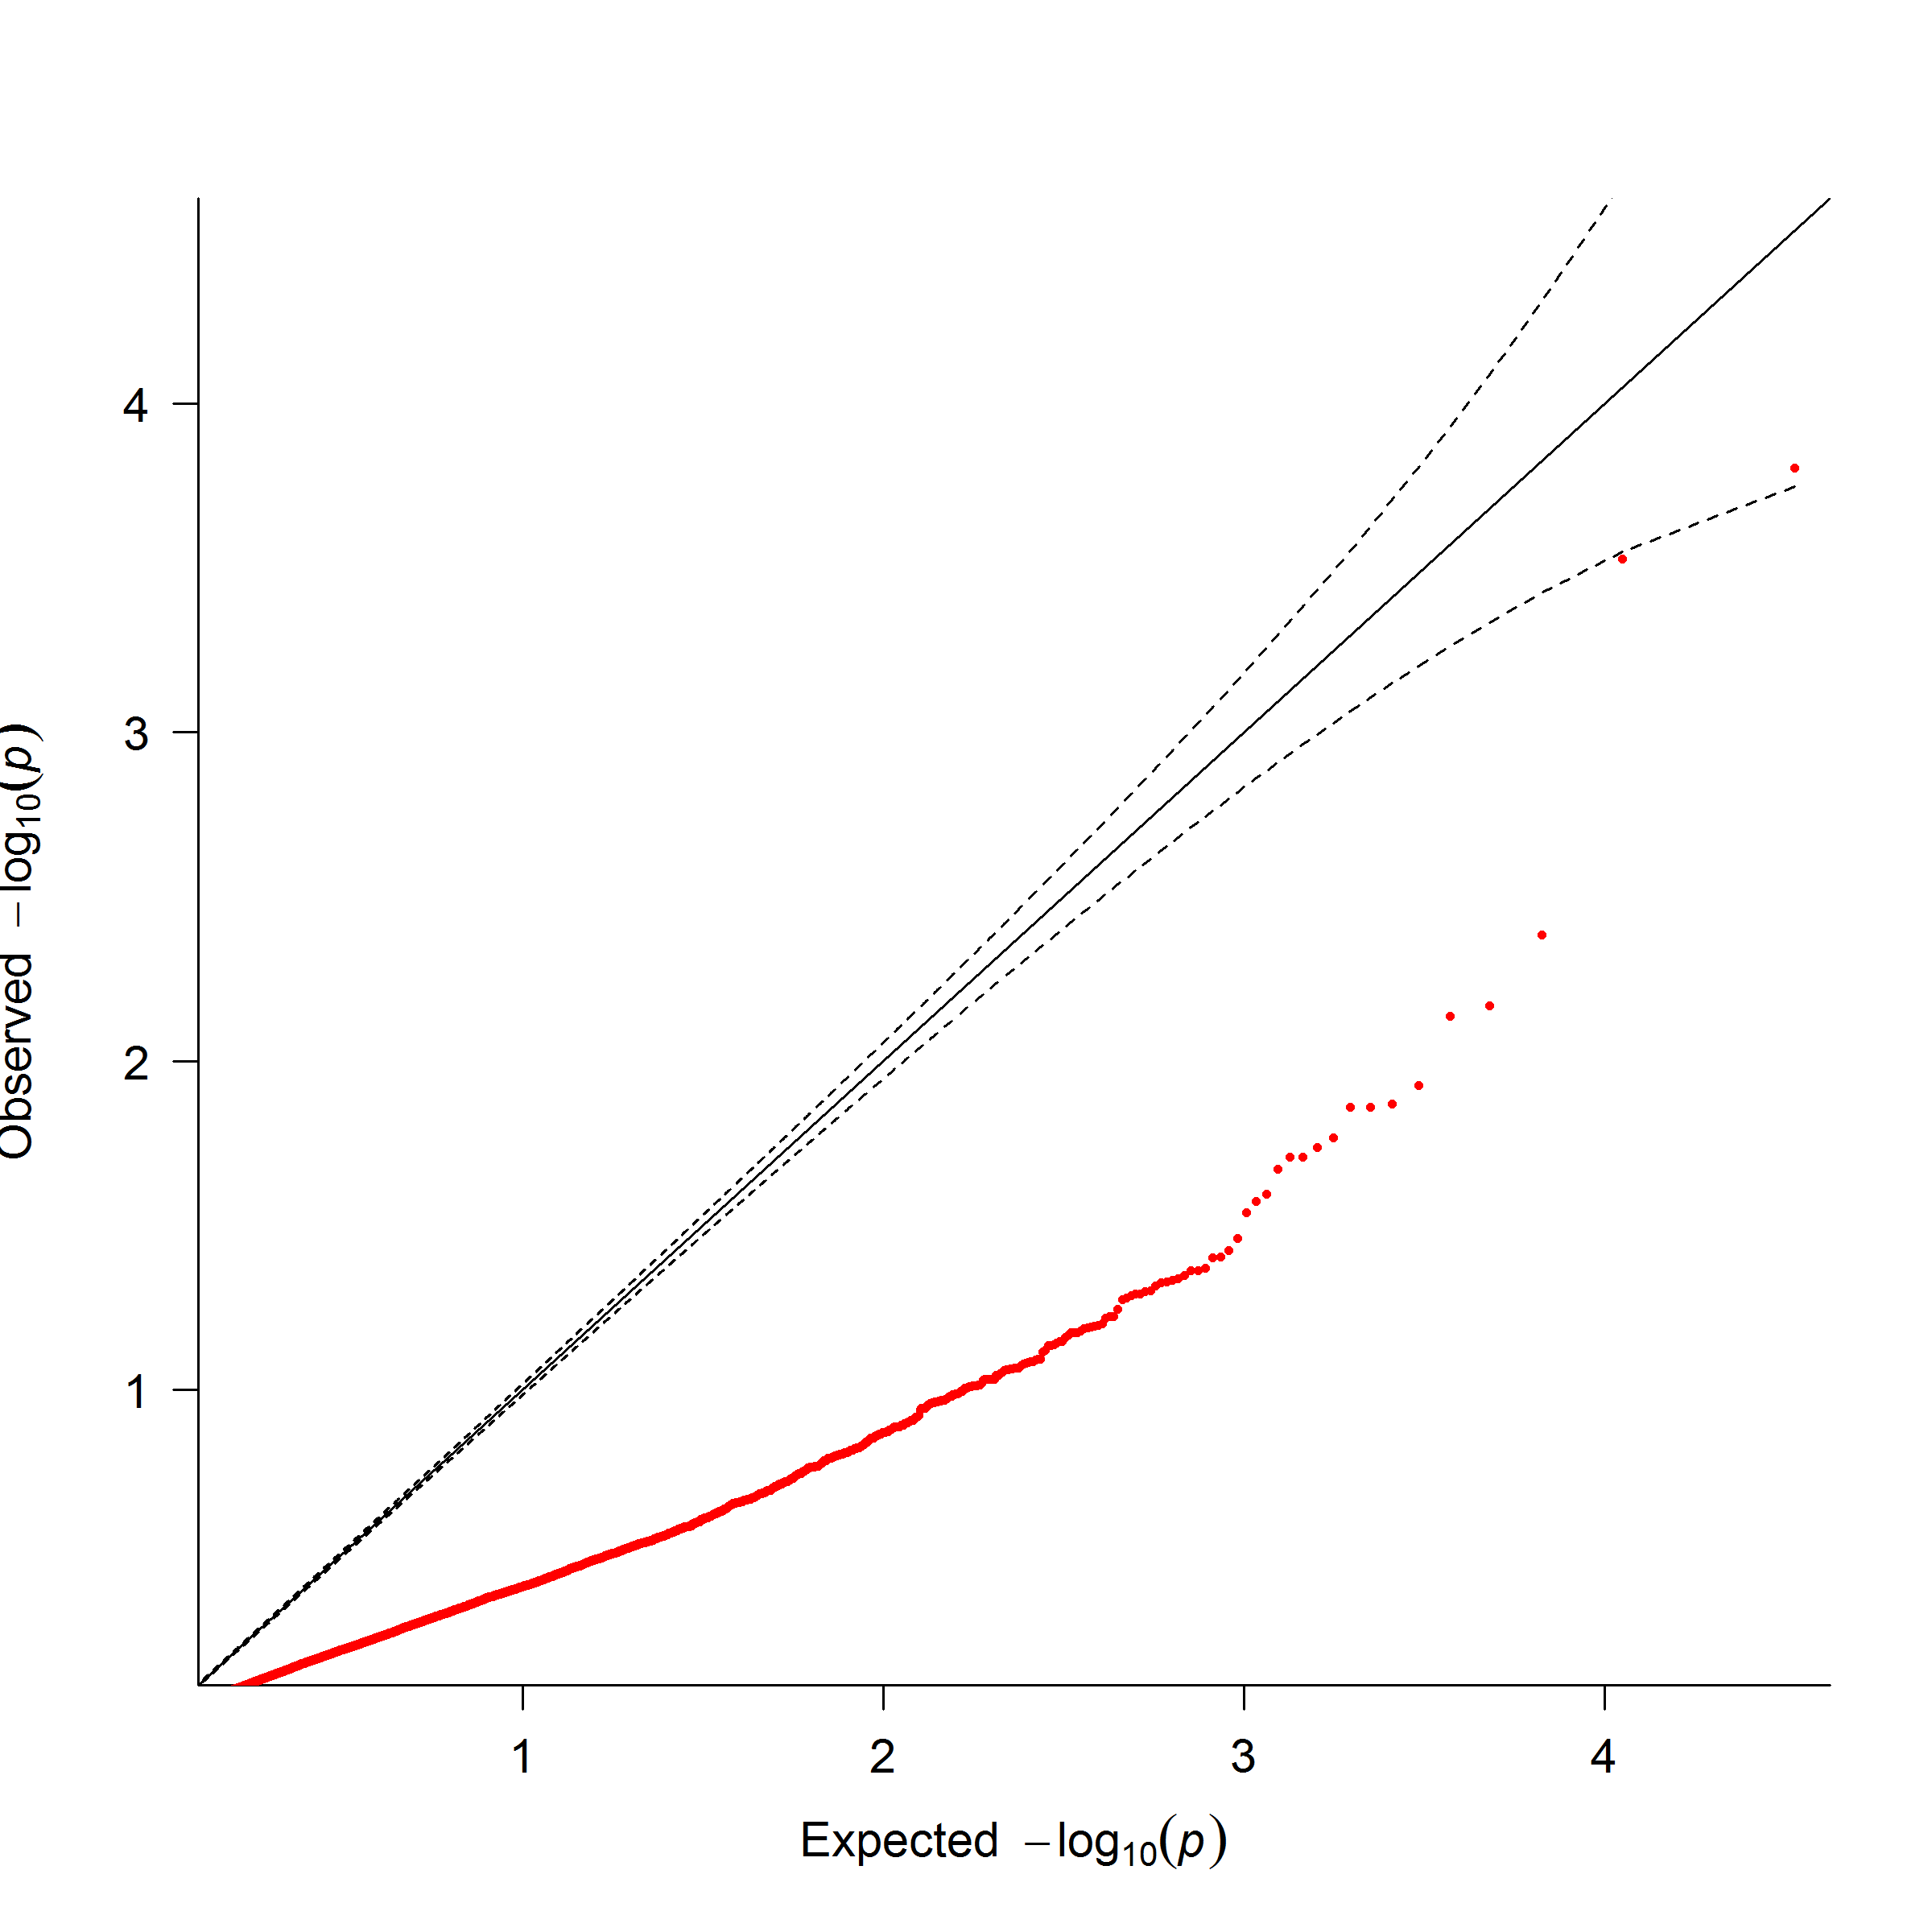
\includegraphics{figure/omega/miaO6_wald_qq.png}}
		\label{fig:miaO6Wald}
	}
	\subfloat[O6-Saline mice vs O3-Saline mice]{
		\scalebox{.4}{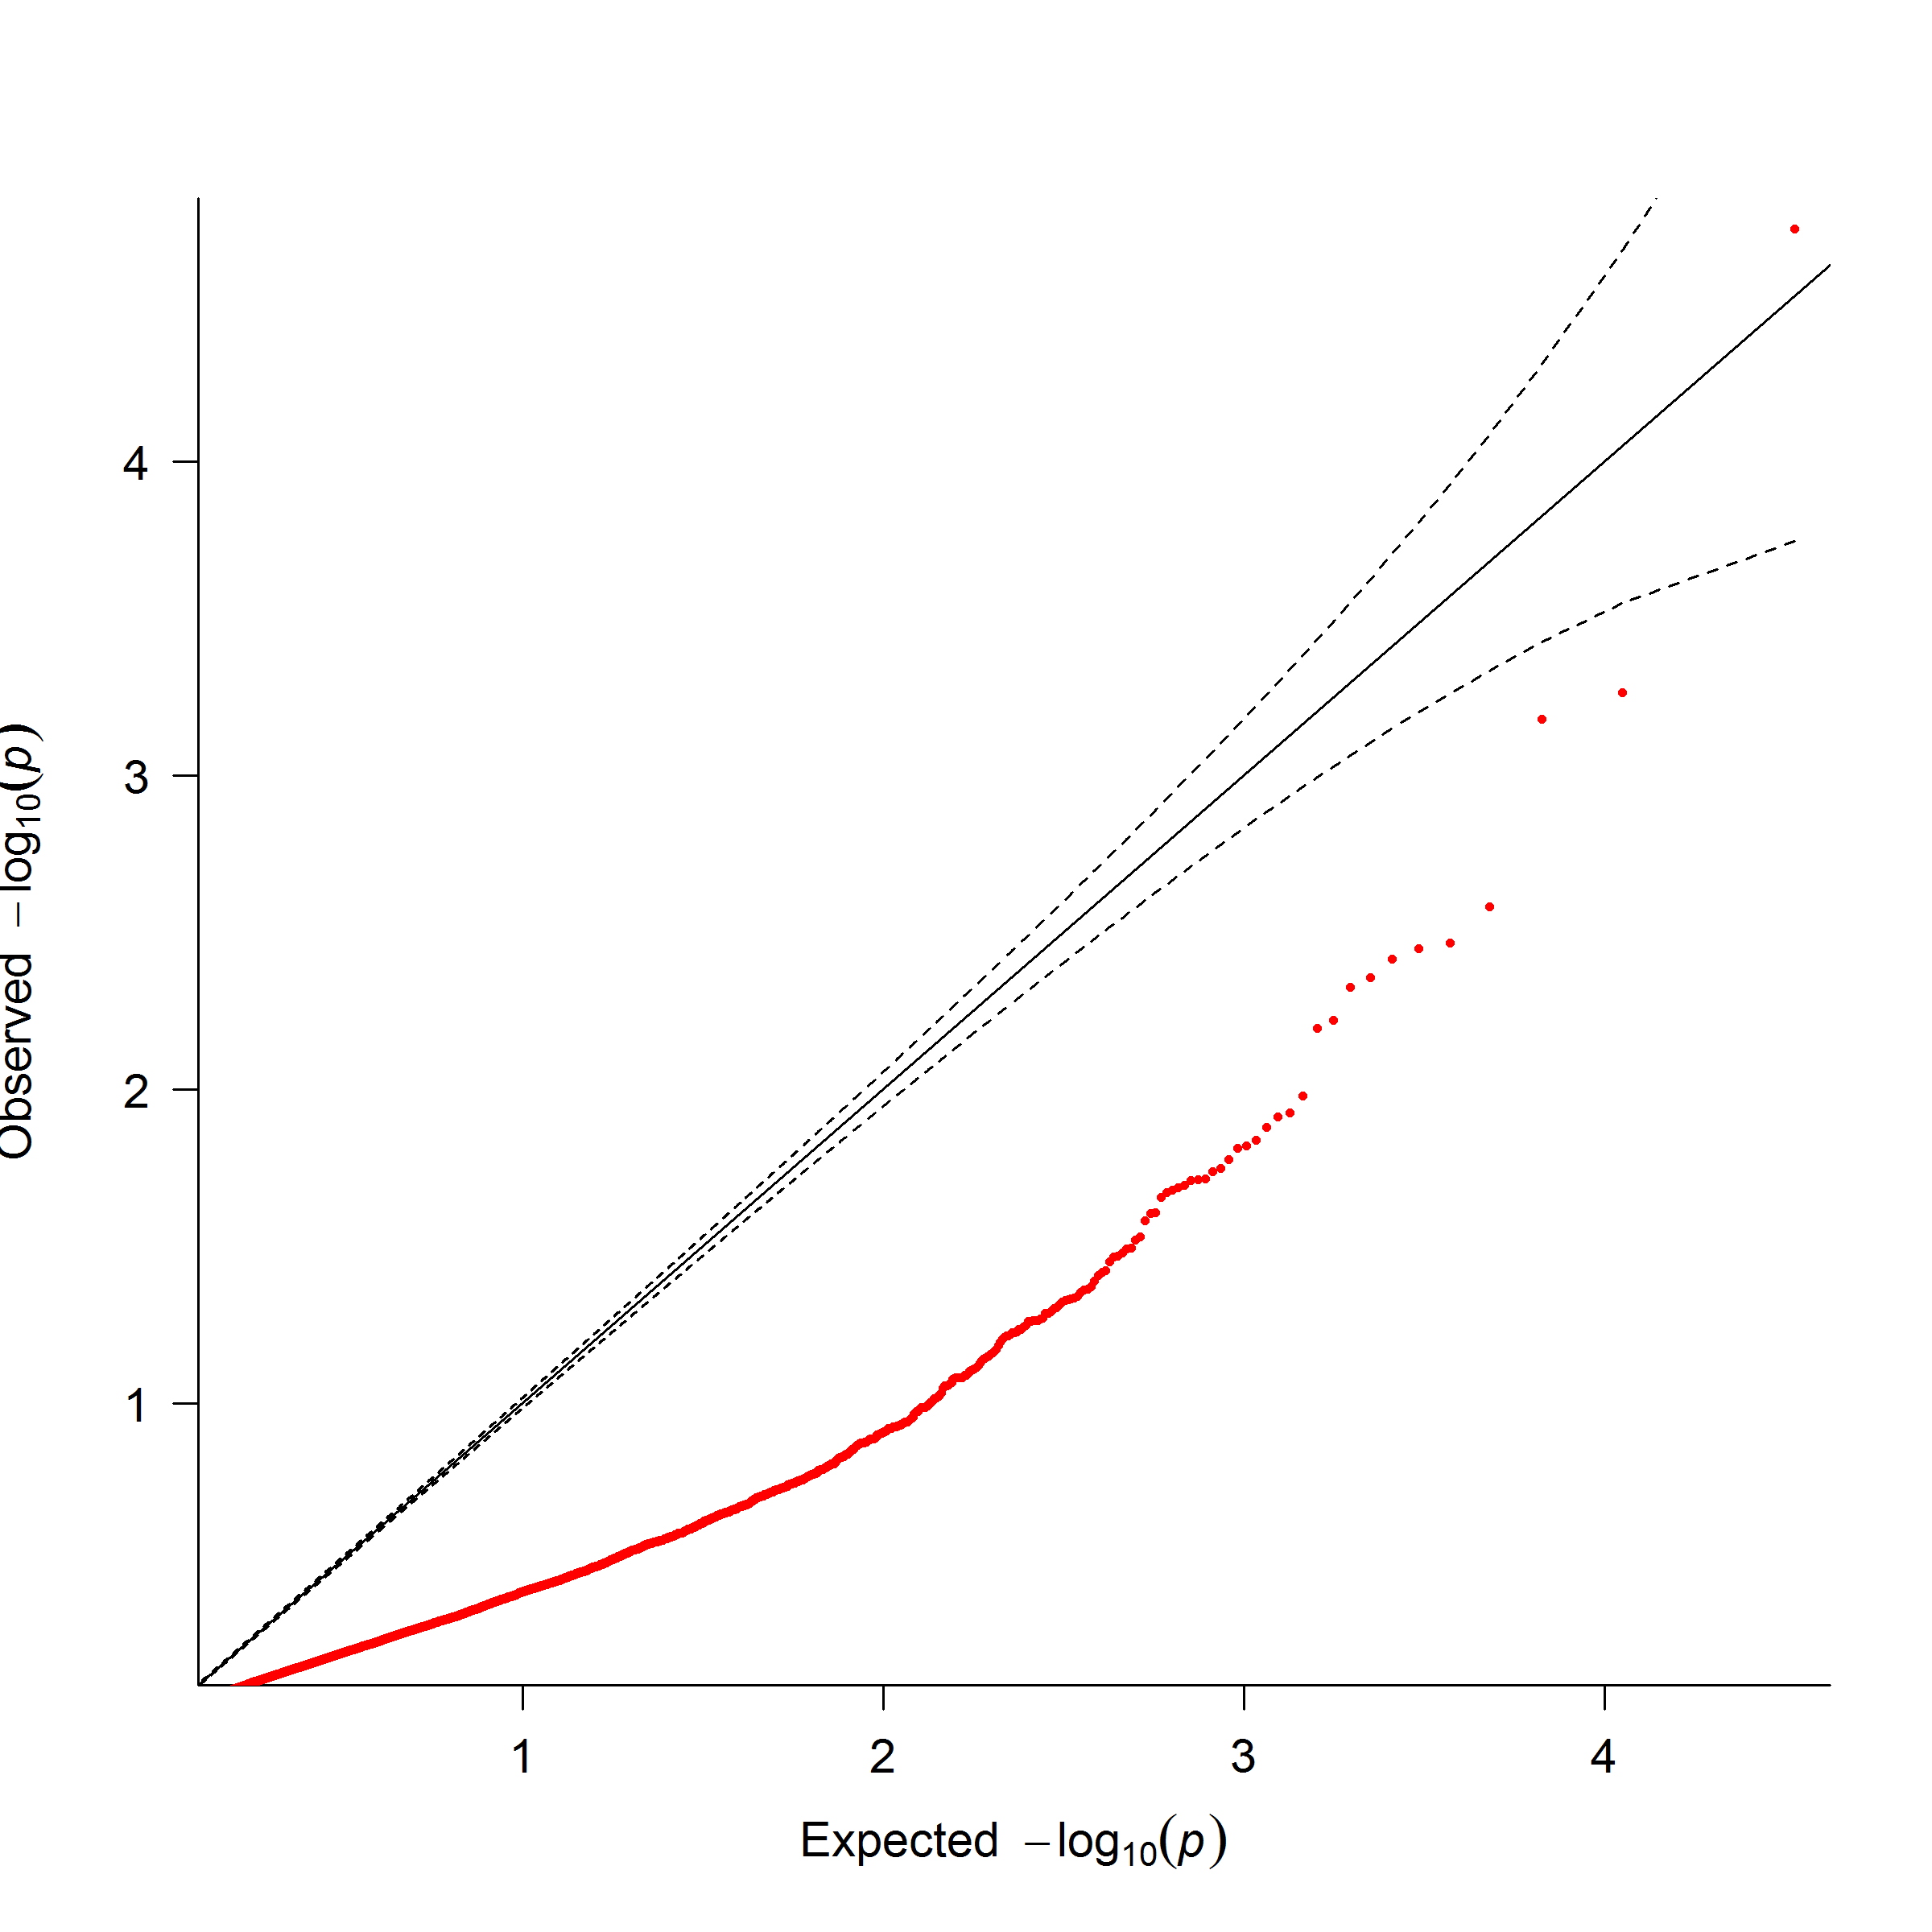
\includegraphics{figure/omega/omegaSAL_wald_qq.png}}
		\label{fig:omegaSALWald}
	}\\
	\subfloat[O6-PolyI:C mice vs O3-PolyI:C mice]{
		\scalebox{.4}{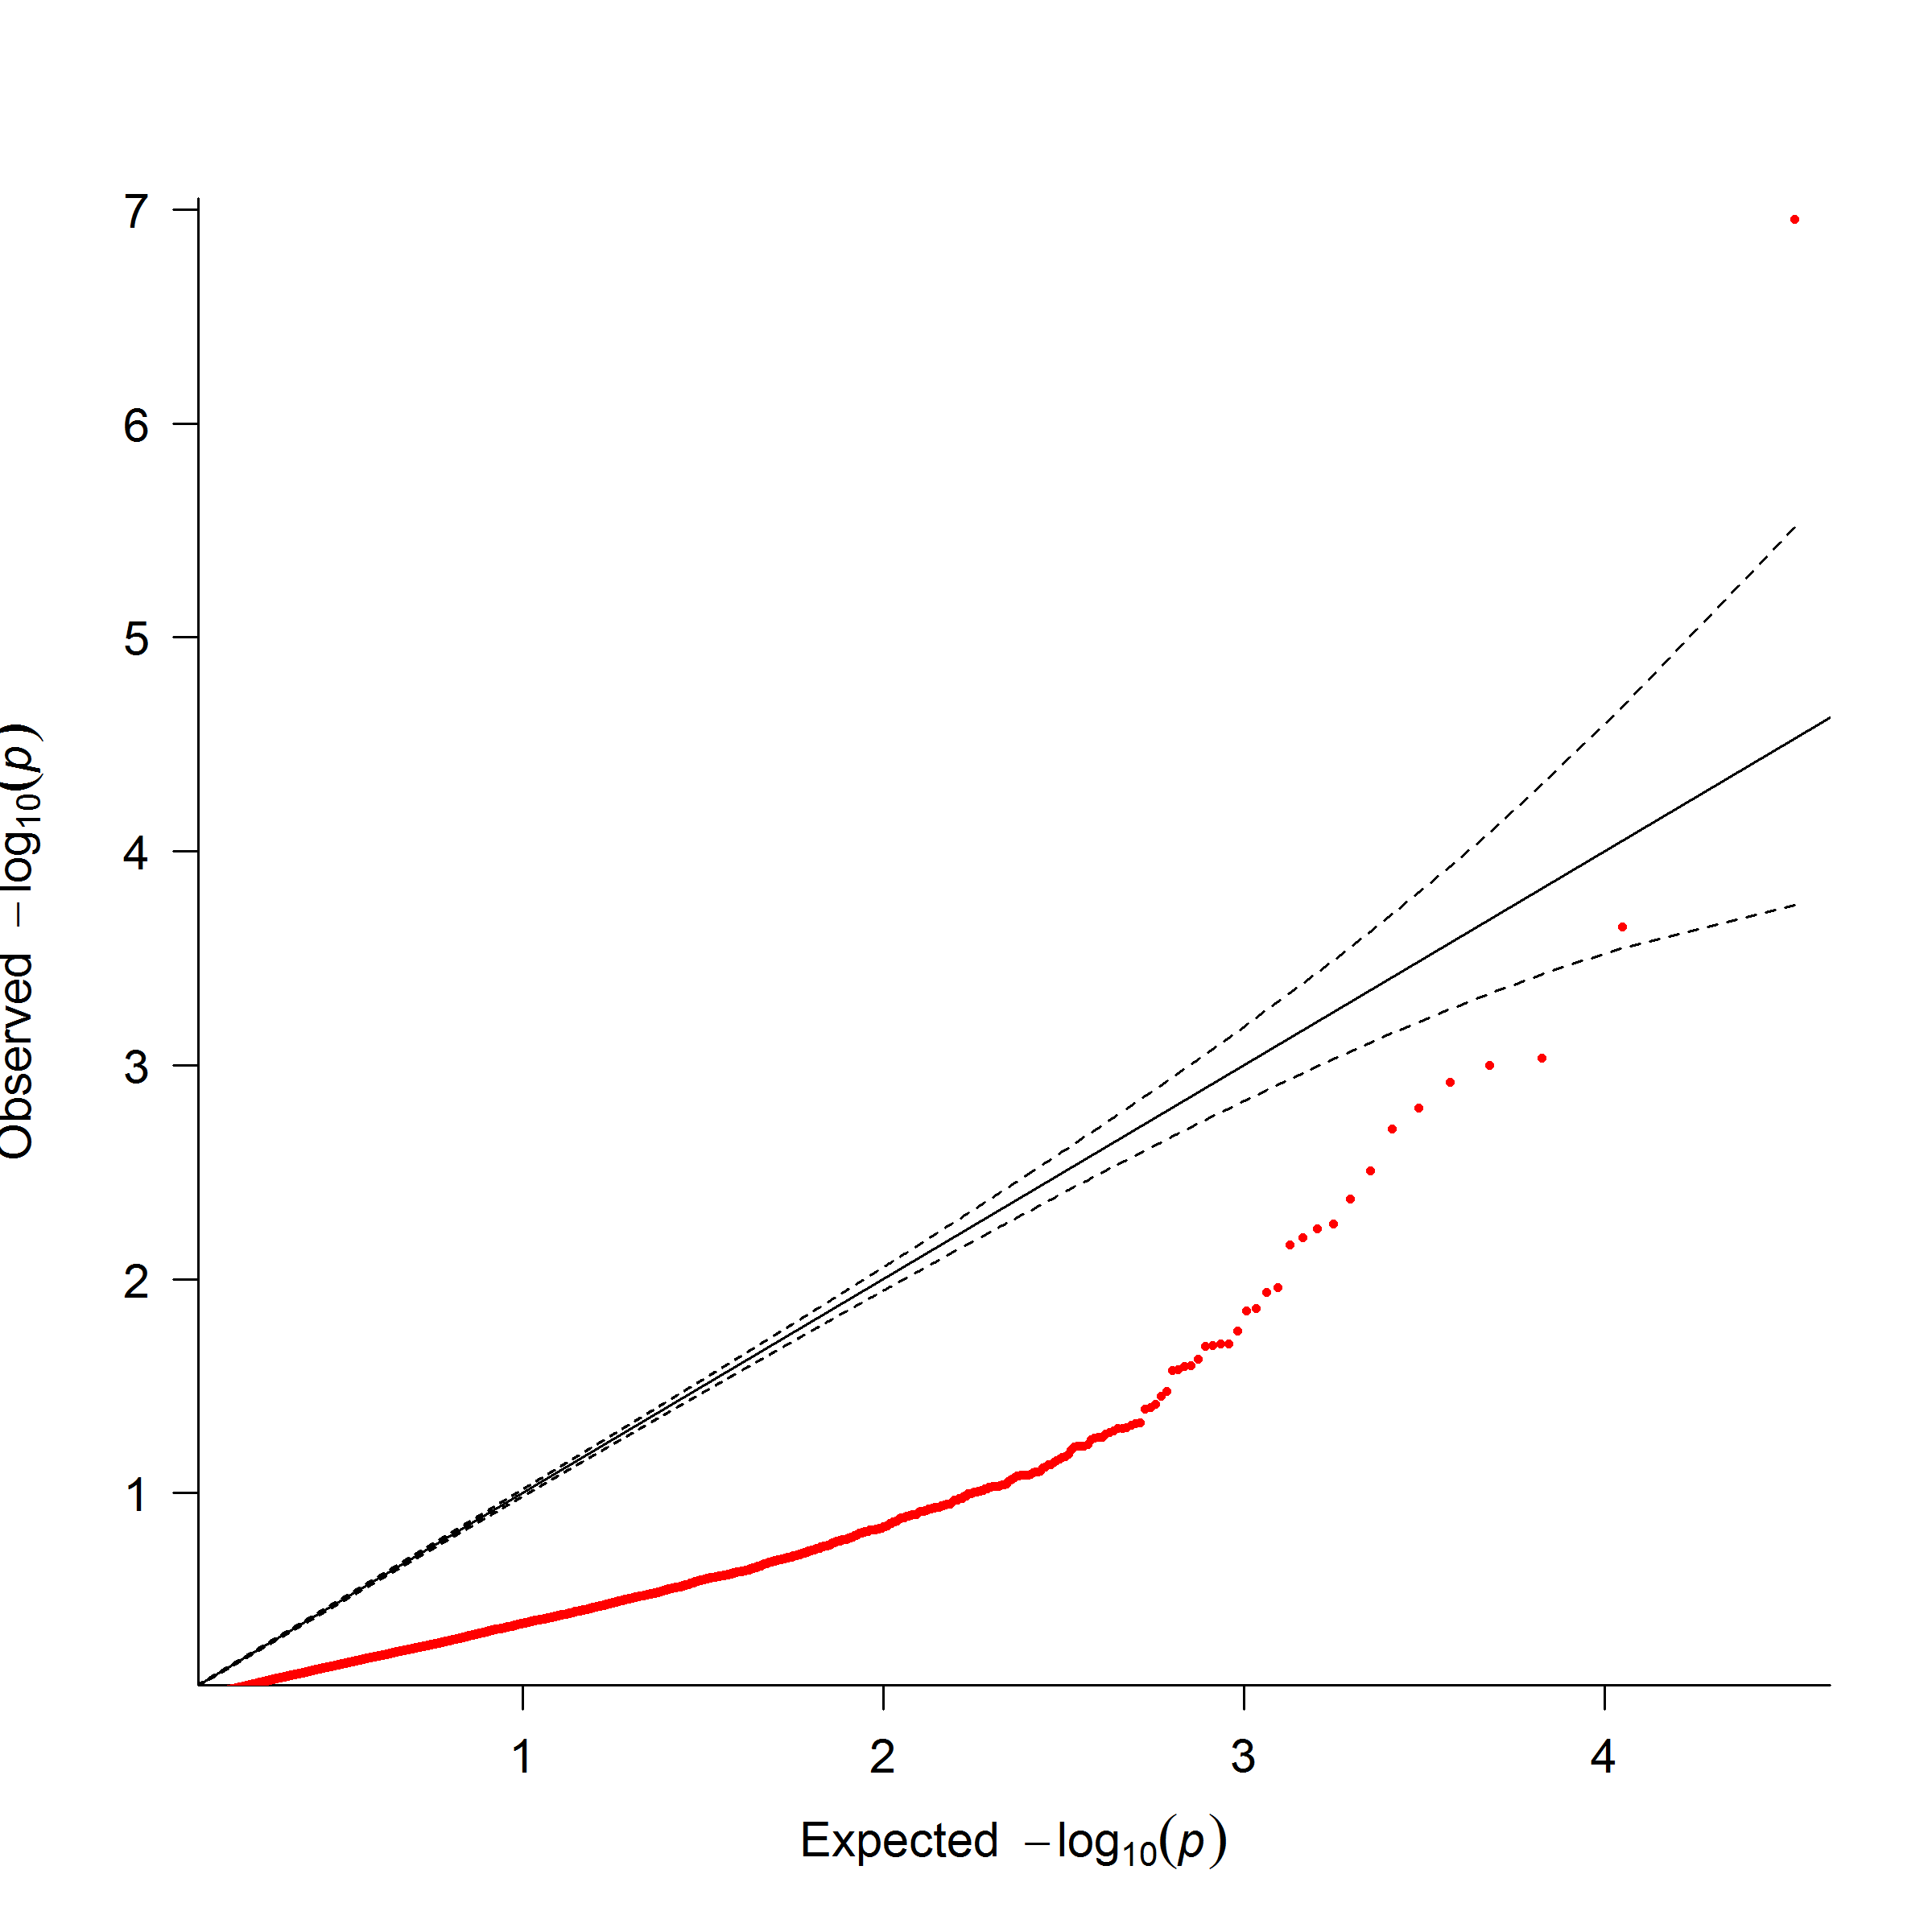
\includegraphics{figure/omega/omegaPOL_wald_qq.png}}
		\label{fig:omegaPOLWald}
	}
%	\subfloat[Batch Effect]{
%		\scalebox{.35}{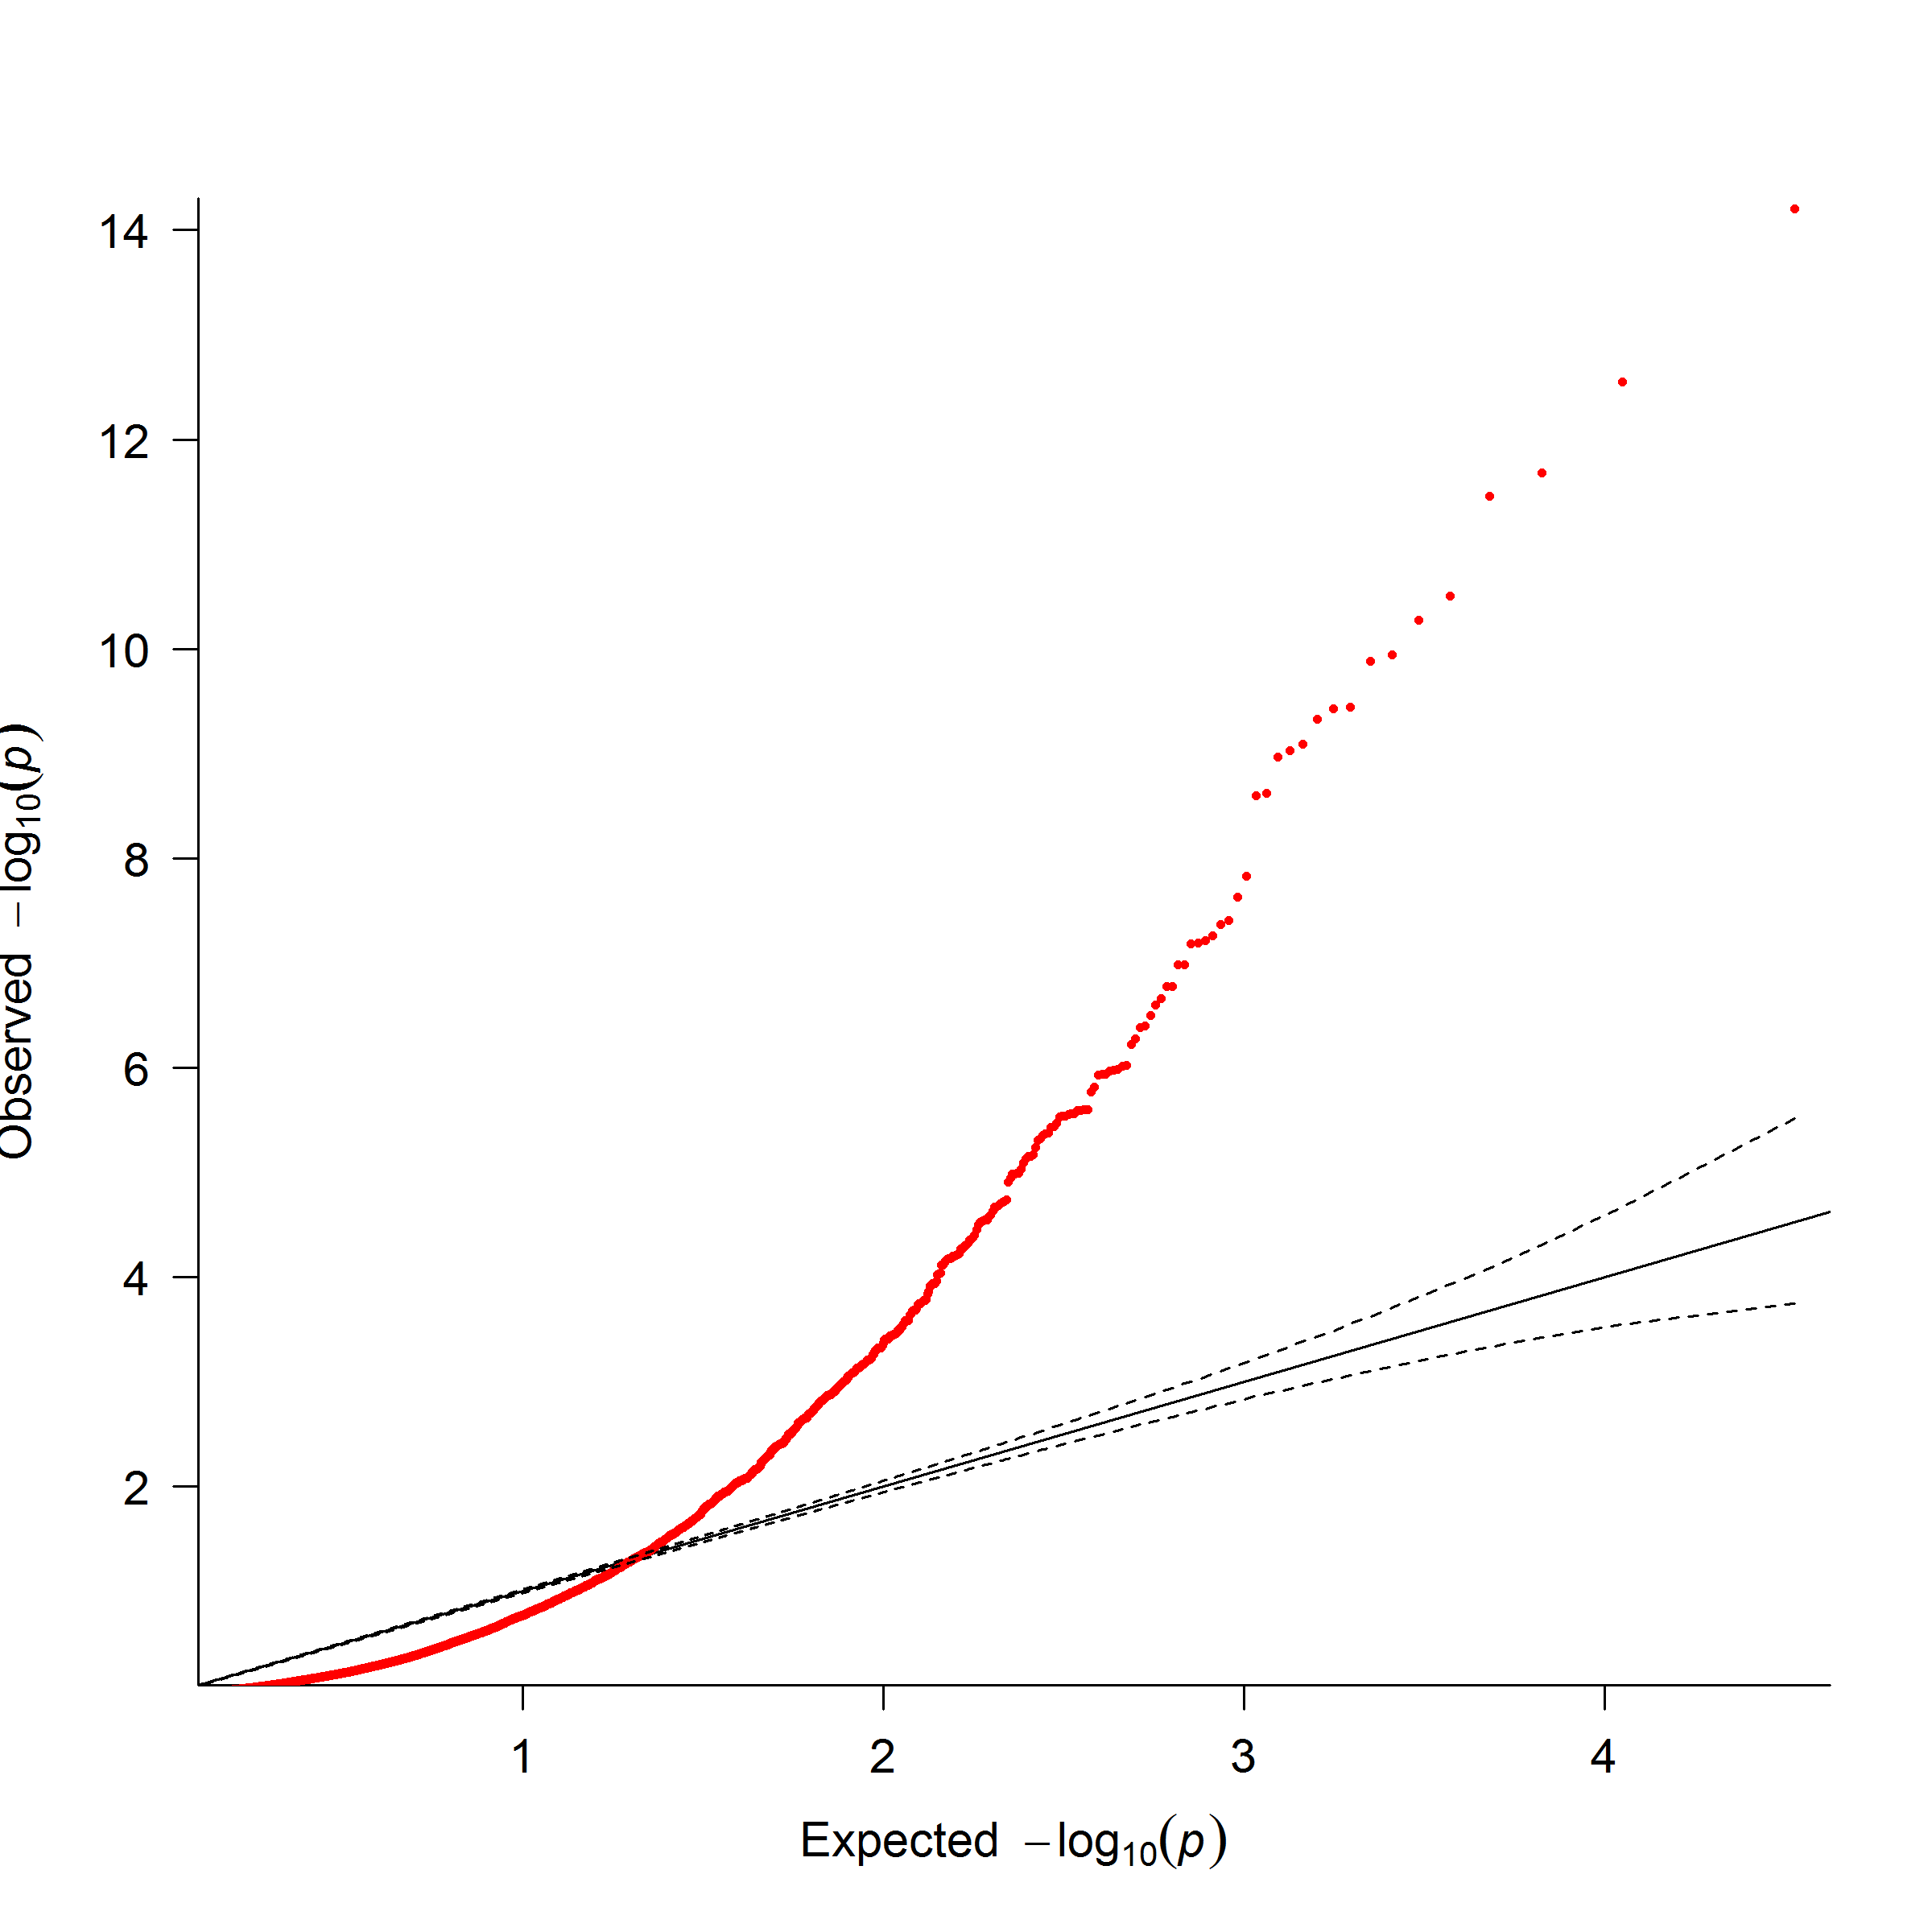
\includegraphics{figure/omega/nobatch_lrt.png}}
%		\label{fig:batchLRT}
%	}
	\caption[QQ Plot Statistic Results]
	{QQ Plot of statistic results.
		From the \gls{qqplot}, it is observed that most of the observed p-values are less than expected. 
		Because the sample size is relatively small, it is likely for the current study to lack detection power, therefore leads to an deflation in p-values.
	
%		Meanwhile, the results from \gls{lrt} suggested that the full model, which adjusted for batch effect, might provide a better fit to our data. 
%		Therefore it is important to adjust for the batch effect. 
		} 
	\label{fig:waldQQ}
\end{figure}
DESeq2 analysis was performed after excluding the problematic sample.
Of the 16,747 genes that passed through quality control, only \textit{Sgk1} (p-adjusted=0.00186) was found to be significantly differentially when comparing the effect of n-3 \gls{pufa} rich diet in \gls{polyic} exposed mice (\cref{fig:omegaPOLWald}).
On the other hand, no significant differentiation is observed in all other comparisons (\cref{fig:miaO6Wald,fig:omegaSALWald}).
%
%\gls{lrt} was performed to test the goodness of fit of model with and without the batch effect include. 
%It is observed that when ``Batch'' was not included in the model, 178 genes are found to be significant (\cref{fig:batchLRT}).
%This indicates that by including ``Batch'' in the statistic model, a significant better fit can be obtained. 

\subsection{Gene Set Analysis}
In total, 7 gene sets were included for the gene set analysis (\cref{tab:genesetRes}).
Of the 7 gene sets tested, 6 are significantly enriched in \gls{mia}, whereas only the \gls{psd} gene set from \gls{go} are significantly enriched in \gls{polyic} exposed mice given the n-3 \gls{pufa} rich diet. 
None of the gene sets are significant in Saline exposed mice given the n-3 \gls{pufa} rich diet. 

For all the gene sets related to \gls{psd}, the \gls{psd} gene set from \citet{Purcell2014} is the only one that is not found to be significant in all conditions.
Upon further investigation, the \gls{psd} gene set from \citet{Purcell2014} is found to be based on the work of \citet{Kirov2012} which includes not only the \gls{psd}, but also \gls{arc}, \gls{nmda} receptor complex and metabotropic glutamate receptor 5 (mGluR5) subsets.

% Table generated by Excel2LaTeX from sheet 'Sheet1'
\begin{landscape}
	\begin{table}
		\centering
		\caption[Results of Gene Set Analysis]{Results of gene set analysis. 
			In total, 7 gene sets were retrieved from \citet{Purcell2014}, \gls{kegg} and \gls{go}. 
			Firstly, Wilcoxon Rank sum test was performed. 
			Except for the \gls{psd} gene set obtained from \citet{Purcell2014}, all pathways are enriched in \gls{mia}.
			On the other hand, the \gls{psd} gene set obtained from \gls{go} is the only gene set that are significantly enriched in \gls{polyic} exposed mice receiving the n-3 \gls{pufa} rich diet, whereas none of the gene sets are significantly enriched in Saline exposed mice receiving the n-3 \gls{pufa} rich diet. 
			Upon further investigation, the \gls{psd} gene set from \citet{Purcell2014} was found to be based on the work of \citet{Kirov2012} which includes not only the \gls{psd}, but also \gls{arc}, \gls{nmda} receptor complex and metabotropic glutamate receptor 5 (mGluR5) subsets.
			The broader definition of the \gls{psd} gene set form \citet{Purcell2014} might explain the difference observed between the \gls{psd} set from \citet{Purcell2014} and \gls{psd} set from \gls{go}.

		}
		\label{tab:genesetRes}%
		%\rowcolors{2}{gray!25}{white}
		\begin{tabular}{lllllllll}
			\toprule
			Gene Set & Source & Size    & Category & \begin{tabular}[t]{@{}c@{}}Diet in \\PolyIC \\Mice\end{tabular}  & MIA Effect   & \begin{tabular}[t]{@{}c@{}}Diet in \\Saline \\Mice\end{tabular} & \begin{tabular}[t]{@{}c@{}}Proportion \\of $h^2$ \\explained\end{tabular} \\%& \begin{tabular}[t]{@{}c@{}}Enrichment \\P-value \end{tabular} \\
			\midrule
			\begin{tabular}[t]{@{}l@{}}Calcium Ion \\Signaling Pathway\end{tabular} & \begin{tabular}[t]{@{}l@{}}KEGG\\(hsa04020)\end{tabular} & 180 & Calcium Ion & 0.0402 & $4.40\times10^{-7}$ & 0.231 & 0.0135 \\%& 0.421 \\
			\rowcolor{gray!25}
			Glutamatergic synapse & \begin{tabular}[t]{@{}l@{}}KEGG\\(hsa04724)\end{tabular} & 114 & PSD   & 0.118 & 0.00490 & 0.123 & 0.0134 \\%& 0.382 \\
			\rowcolor{white}
			\begin{tabular}[t]{@{}l@{}}Voltage-Gated Calcium \\Channel Activity\end{tabular} & \begin{tabular}[t]{@{}l@{}}GO\\(GO:05245)\end{tabular}    & 44 & Calcium Ion & 0.0262 & $3.45\times10^{-6}$ & 0.137 & 0.00771 \\%& 0.313 \\
			\rowcolor{gray!25}
			Calcium Channel Activity & \begin{tabular}[t]{@{}l@{}}GO\\(GO:05262)\end{tabular}   & 111 & Calcium Ion & 0.0942 & 0.00209 & 0.0880 & 0.0119 \\%& 0.593 \\
			\rowcolor{white}
			PSD   & \begin{tabular}[t]{@{}l@{}}GO\\(GO:14069)\end{tabular}   & 194 & PSD   & $4.86\times10^{-3}$ & $6.31\times10^{-9}$ & 0.0383 & 0.0352 \\%& 0.00624 \\
			\rowcolor{gray!25}
			PSD   & Purcell &   685    & PSD   & 0.113 & 0.328 & 0.977 & 0.0486 \\%& 0.131 \\
			\rowcolor{white}
			\Glng{scz} GWAS  & Purcell &  479     & GWAS  & 0.3048 & $6.91\times10^{-3}$ & 0.551 & 0.0998 \\%& $7.42\times10^{-8}$ \\
			\bottomrule
		\end{tabular}%
	\end{table}%
\end{landscape}

\subsection{Partitioning of Heritability}
It is observed that all calcium ion channel gene sets accounts for around 0.77-1.35\% of the \gls{SNP} heritability of \glng{scz}, whereas the \gls{psd} gene sets contribute 1.34\% to 4.86\%.

Finally, the \glng{scz} \gls{GWAS} gene set contribute most to the \gls{SNP} heritability of \glng{scz}, contributing 9.9\% of the \gls{SNP} heritability.
%
%\subsection{Functional Annotation}
%It is common practice to perform functional annotation to the \glspl{deg}. 
%However, in most of our analysis, there were either no \gls{deg} or only 1 \gls{deg}, making it difficult to perform functional annotation.
%We therefore used the Wilcox rank sum test to analysis whether if a pathway contain genes that are more significant than genes not within the pathway.
%
%None of the pathways were found to be significant when comparing the effect of the n-3 \gls{pufa} rich diet in Saline exposed mice. 
%On the contrary, 17 pathways were found significant when comparing the effect of n-3 \gls{pufa} rich diet in \gls{polyic} exposed samples (\cref{tab:o6polyPath}) where 4 pathways were related to growth factors such as \gls{fgf} or \gls{egf} and 4 others were related to kinases such as \gls{pi3k} or \gls{mapk}.
%
%Finally, 12 pathways were found to be significant when comparing Saline and \gls{polyic} exposed mice given the n-6 \gls{pufa} rich diet (\cref{tab:miaPath}) with pathways such as neuroactive ligand-receptor interaction (p-adj = $1.27\times10^{-3}$), calcium signaling pathway (p-adj = $2.79\times10^{-3}$) and genes involved in Neuronal System (p-adj=0.00153) among the significant pathways.
%
%\subsection{Partitioning of Heritability}
%Given the significant pathways, we performed the partitioning of heritability using \gls{ldsc} \citep{Bulik-Sullivan2015}.
%In total, 14 unique pathways were included in the analysis were 4 of them were found to have non-negative contribution to the heritability of \glng{scz}, including the pathway related to neuronal system, \gls{ecm} glycoprotein, calcium signaling and \gls{mapk} signaling (\cref{tab:partitioning}).
%All of these pathways were affected by \gls{mia} and only the \gls{ecm} pathways were also found to be affected by n-3 \gls{pufa} rich diet in \gls{polyic} exposed mice.
%Moreover, the ``super pathway'' for \gls{mia} were found to be significant (p-value=0.0402) yet the ``super pathway'' for diet was found to be insignificant (p-value=0.414).

\subsection{Designing the Replication Study}
Using Scotty \citep{Busby2013}, it is estimated that a minimal of 10 samples per group are required for the follow-up study in order to obtain the desirable power. 

%
%\begin{landscape}
%	\begin{table}
%		\begin{tabular}{rrrp{10cm}r}
%			\toprule
%			ID&	Size&	Source&	Description&	Adjusted P-Value\\
%			\midrule
%			M508&	78&	REACTOME&	Genes involved in Signaling by SCF-KIT&	0.00671\\
%			M570&	44&	REACTOME&	Genes involved in PI3K events in ERBB2 signaling&	0.0242\\
%			M3008&	196&	NABA&	Genes encoding structural ECM glycoproteins&	0.0309\\
%			M1090&	112&	REACTOME&	Genes involved in Signaling by FGFR&	0.0309\\
%			M563&	109&	REACTOME&	Genes involved in Signaling by EGFR in Cancer&	0.0309\\
%			M17776&	100&	REACTOME&	Genes involved in Downstream signaling of activated FGFR&	0.0309\\
%			M1076&	83&	REACTOME&	Genes involved in Amyloids&	0.0309\\
%			M850&	56&	REACTOME&	Genes involved in PI-3K cascade&	0.0309\\
%			M10450&	38&	REACTOME&	Genes involved in GAB1 signalosome&	0.0309\\
%			M16227&	24&	REACTOME&	Genes involved in Cholesterol biosynthesis&	0.0309\\
%			M5872&	17&	KEGG&	Steroid biosynthesis&	0.0309\\
%			M16334&	10&	BIOCARTA&	Eph Kinases and ephrins support platelet aggregation&	0.0309\\
%			M5884&	275&	NABA&	Ensemble of genes encoding core extracellular matrix including ECM glycoproteins, collagens and proteoglycans&	0.0456\\
%			M635&	127&	REACTOME&	Genes involved in Signaling by FGFR in disease&	0.0456\\
%			M568&	38&	REACTOME&	Genes involved in PI3K events in ERBB4 signaling&	0.0456\\
%			M165&	32&	PID&	Syndecan-4-mediated signaling events&	0.0456\\
%			M1262&	15&	REACTOME&	Genes involved in GRB2:SOS provides linkage to MAPK signaling for Intergrins&	0.0456\\
%			\bottomrule
%		\end{tabular}
%		\caption[Significant Pathways When Comparing Effect of Diet in PolyI:C Exposed Mouse]{Significant Pathways when comparing effect of diet in \gls{polyic} exposed mice.
%			The pathway IDs are the systematic name from \gls{msigdb}.
%			Most of the significant pathways were related to the kinase such as PI3K and MAPK or growth factors such as \gls{fgf} and \gls{egf}.
%		}
%		\label{tab:o6polyPath}
%	\end{table}
%	
%	\begin{table}
%		\begin{tabular}{rrrp{10cm}r}
%			\toprule
%			ID&	Size&	Source&	Description&	Adjusted P-Value\\
%			\midrule
%			M13380&	272&	KEGG&	Neuroactive ligand-receptor interaction&	$1.27\times10^{-3}$\\
%			M2890&	178&	KEGG&	Calcium signaling pathway&	$2.79\times10^{-3}$\\
%			M12289&	188&	REACTOME&	Genes involved in Peptide ligand-binding receptors&	0.00118\\
%			M5884&	275&	NABA&	Ensemble of genes encoding core extracellular matrix including ECM glycoproteins, collagens and proteoglycans&	0.00119\\
%			M735&	279&	REACTOME&	Genes involved in Neuronal System&	0.00153\\
%			M15514&	186&	REACTOME&	Genes involved in Transmission across Chemical Synapses&	0.00401\\
%			M4904&	121&	REACTOME&	Genes involved in G alpha (s) signalling events&	0.0127\\
%			M3008&	196&	NABA&	Genes encoding structural ECM glycoproteins&	0.0131\\
%			M752&	137&	REACTOME&	Genes involved in Neurotransmitter Receptor Binding And Downstream Transmission In The Postsynaptic Cell&	0.0131\\
%			M10792&	267&	KEGG&	MAPK signaling pathway&	0.0195\\
%			M17&	59&	PID&	Notch signaling pathway&	0.0406\\
%			M18437&	184&	REACTOME&	Genes involved in G alpha (q) signalling events&	0.0406\\
%			\bottomrule
%		\end{tabular}
%		\caption[Significant Pathways When Comparing Effect of PolyI:C in Mouse Given n-6 \gls{pufa} Rich Diet]{Significant pathways when comparing effect of PolyI:C in mouse given n-6 \gls{pufa} rich diet.
%			The pathway IDs are the systematic name from \gls{msigdb}.
%			Interestingly, we observed a lot of neural related pathways and even got significant signal in the calcium signaling pathway, which was reported to be associated with \glng{scz} \citep{Purcell2014}. 
%		}
%		\label{tab:miaPath}
%	\end{table}
%	
%	\begin{table}
%		\begin{tabular}{rrrp{9cm}p{1.7cm}p{1.5cm}p{1.7cm}}
%			\toprule
%			ID& Size&	Source&	Description&	Proportion of $h^2$&	SE&	Enrichment Q-Value\\
%			\midrule
%			M735&	279&	REACTOME&	Genes involved in Neuronal System&	0.0287&	0.00627&	0.0456\\
%			M5884&	275&	NABA&	Ensemble of genes encoding core extracellular matrix including ECM glycoproteins, collagens and proteoglycans&	0.00363&	0.00342&	0.0456\\
%			M2890&	178&	KEGG&	Calcium signaling pathway&	0.0260&	0.00856&	0.127\\
%			M10792&	267&	KEGG&	MAPK signaling pathway&	0.0257&	0.008713&	0.127\\	
%			\bottomrule
%		\end{tabular}
%		\caption[Pathways Significantly Contributes to SNP Heritability of Schizophrenia.]{Pathways significantly contributes to \gls{SNP} heritability of \glng{scz}.
%		}
%		\label{tab:partitioning}
%	\end{table}
%\end{landscape}

\section{Discussion}
\subsection{Serine/threonine-protein kinase}
Our results demonstrated that the expression of Serine/threonine-protein kinase \textit{Sgk1} in the cerebellum of \gls{polyic} exposed mice might have been affected by n-3 \gls{pufa} rich diet.
\textit{Sgk1} is a serine/threonine kinase activated by \gls{pi3k}/Akt signaling.
Studies have reported that the expression of \textit{Sgk1} is associated with spatial learning, fear-conditioning learning and recognition learning in rat \citep{Tsai2002,Lee2003}.
For example, \citet{Tsai2002} observed a 4 fold increase of \textit{Sgk1} in the hippocampus of fast learners when compared to slow learners.
Furthermore, the transfection of \textit{Sgk1} mutant DNA impairs the water maze performance in rat \citep{Tsai2002}.

On the other hand, it was found that \textit{Sgk1} can regulates the AMPA and kainate glutamate receptors, especially GluR6, which is encoded by \textit{Grik2} \citep{Lang2006,Lang2010}.
The kainate receptors contribute to the excitatory postsynaptic current and are important to the synaptic transmission and plasticity in the hippocampus \citep{Lang2006}.
The upregulation of AMPA and kainate receptors are therefore expected to enhance the excitatory effects of glutamate \citep{Lang2010}.

Furthermore, \textit{Sgk1} can up-regulates the glutamate transporters such as EAAT4 \citep{Bohmer2004}, which are vital for the clearance of glutamate from the synaptic cleft.
This prevents excessive glutamate accumulation, thus help to prevent the neurotoxic effects of glutamate \citep{Lang2010}.
In addition, \citet{Schoenebeck2005} demonstrated that \textit{Sgk1} has a neuroprotective role in oxidative stress situations. 
Together, the evidences suggest that \textit{Sgk1} has an important role in the regulation of the glutamatergic system.
An increase in expression of \textit{Sgk1} might help to improve normal functioning of the glutamatergic system.

\begin{figure}
	\centering
	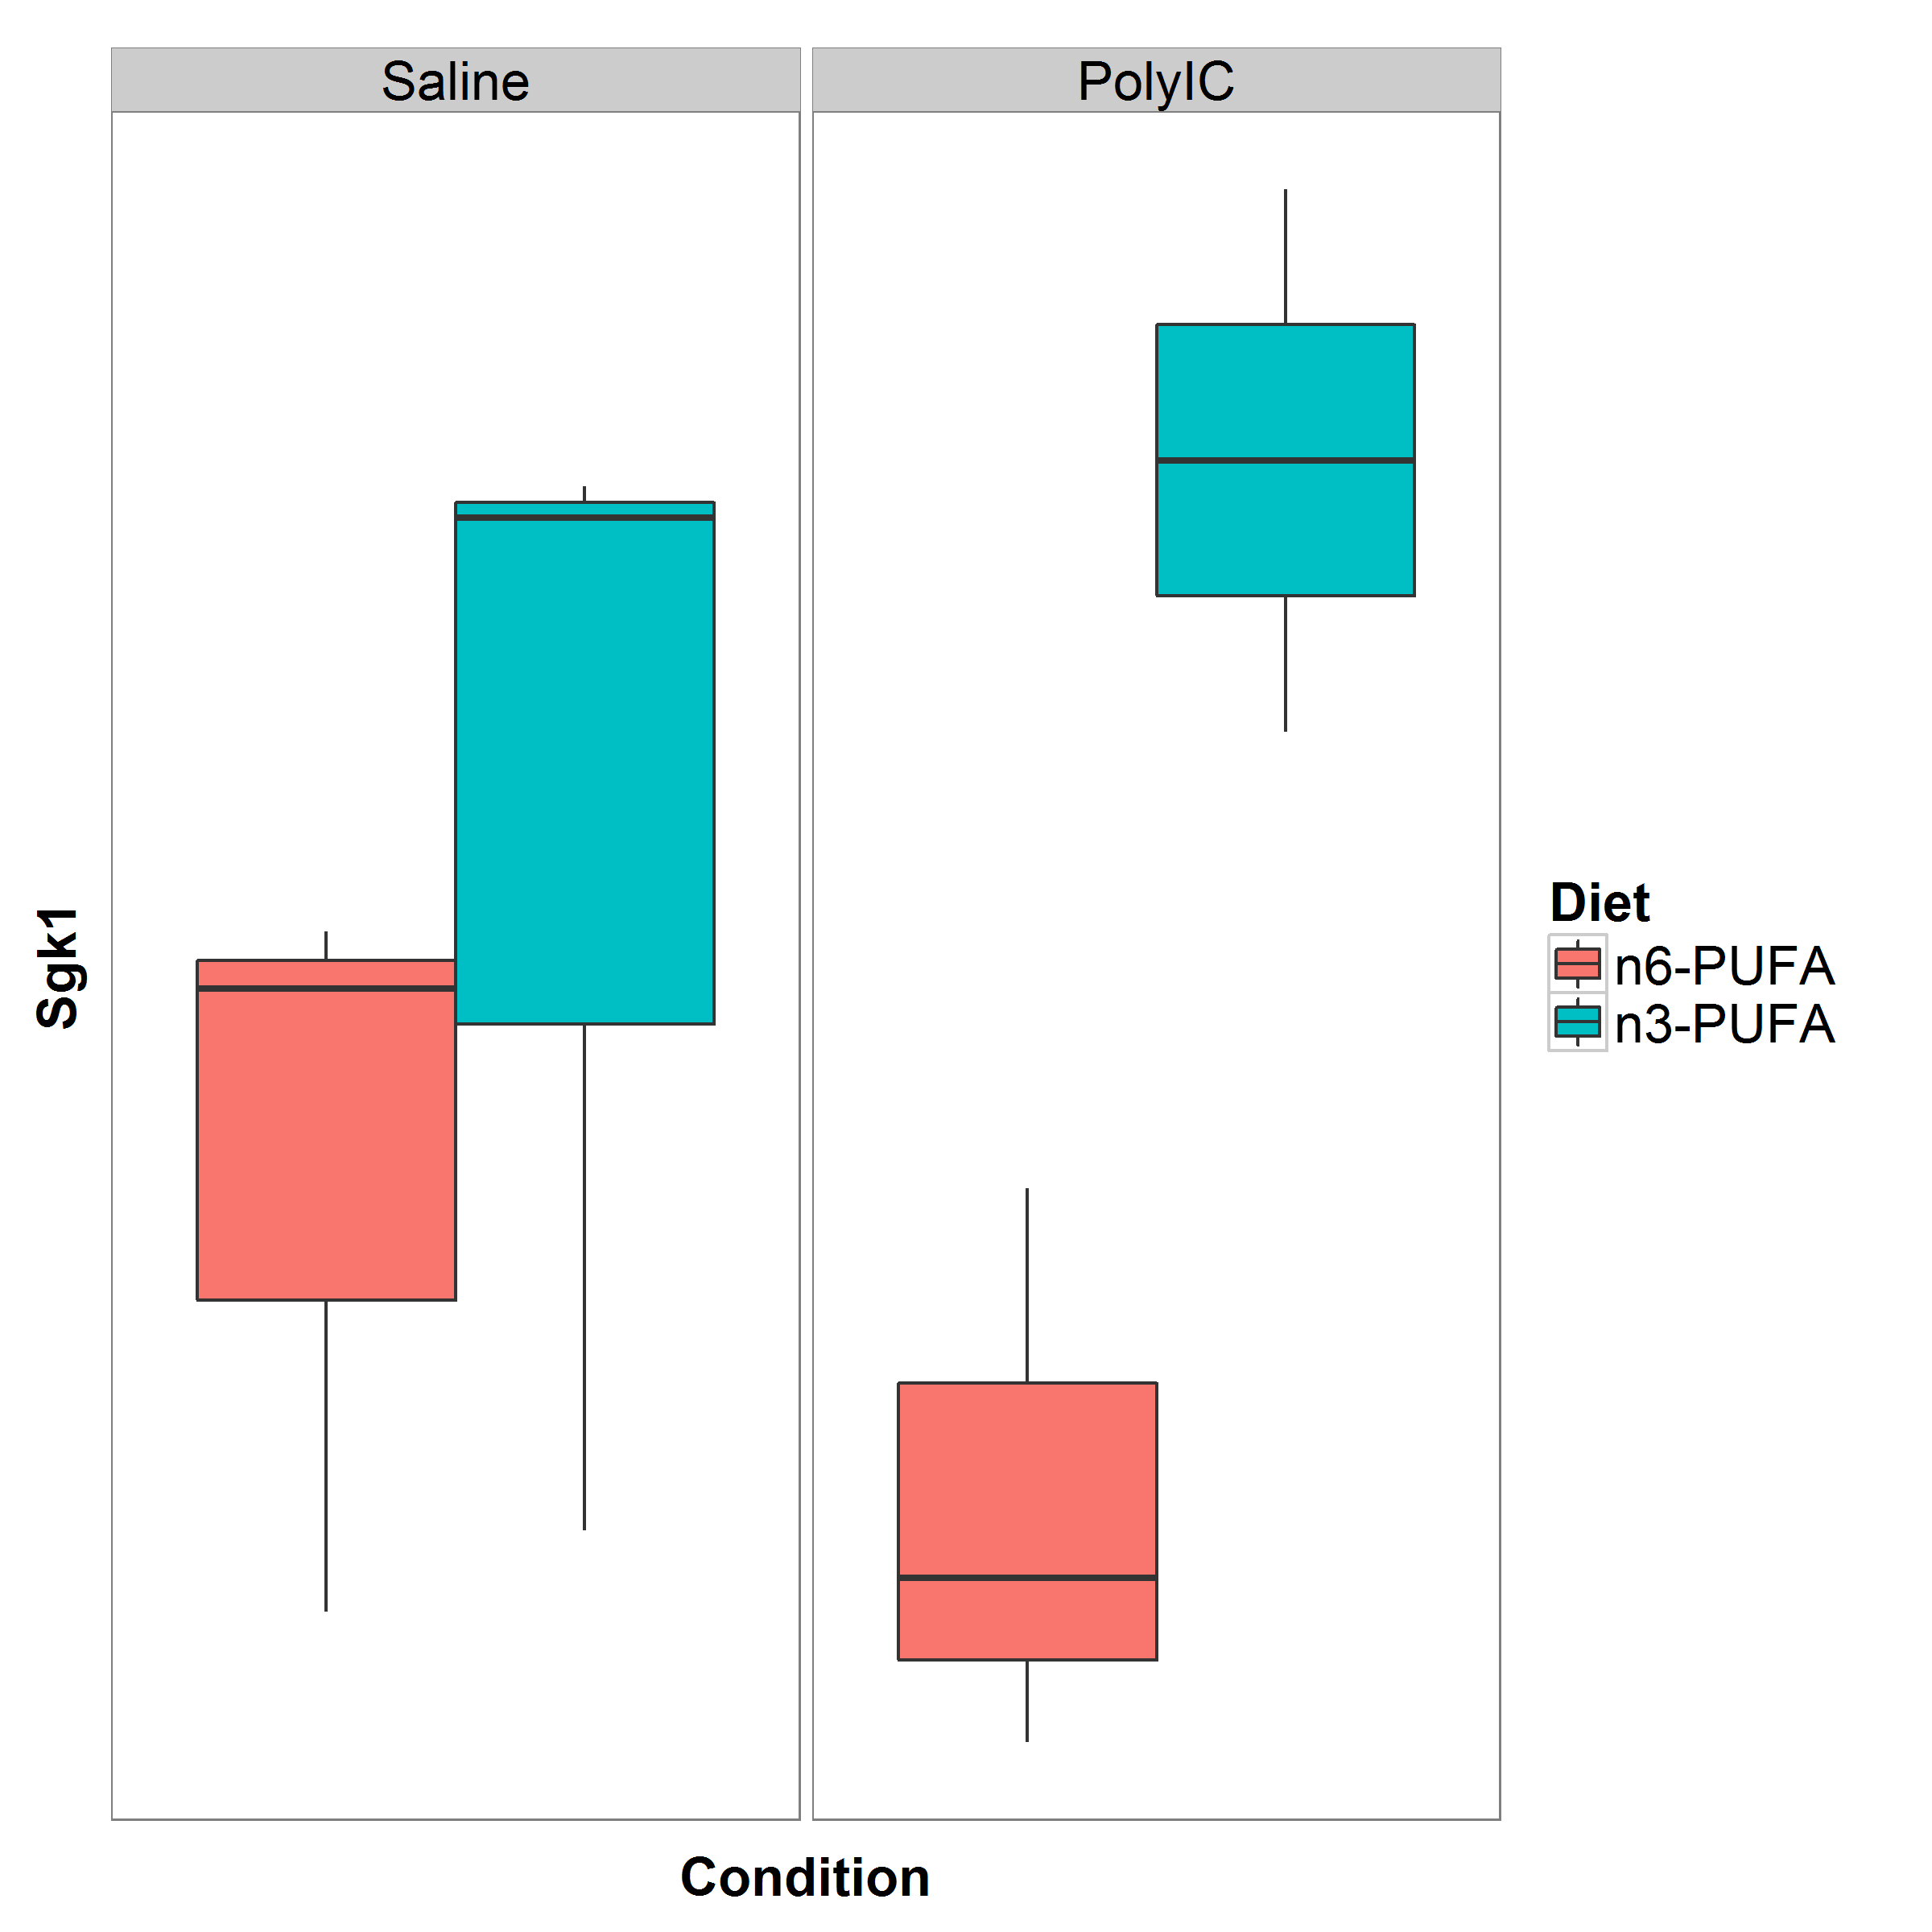
\includegraphics[width=0.6\textwidth]{figure/omega/Sgk1_expression.png}
	\caption[Normalized Expression of \textit{Sgk1}]{
		Normalized Expression of \textit{Sgk1}.
		It was observed that the expression level of \textit{Sgk1} increases after the mice was given a n3-\gls{pufa} rich diet where a significant increase was observed in mice exposed to \gls{polyic}.
	}\label{fig:sgk1Express}
\end{figure}

Interestingly although the expression of \textit{Sgk1} is lower in the \gls{polyic} exposed samples when compared to the Saline exposed samples (\cref{fig:sgk1Express}), the difference is insignificant (unadjusted p-value=0.0254, q-value = 0.999). 
A significant difference is only observed when comparing the effect of n-3 \gls{pufa} rich diet and the control diet in \gls{polyic} exposed mice.
The expression of \textit{Sgk1} is significantly higher in \gls{polyic} exposed samples who received the n-3 \gls{pufa} rich diet. 
Although there is no direct evidence linking n-3 \gls{pufa} diet with the expression of \textit{Sgk1}, \citet{Zhang2015} demonstrated that n-3 \gls{pufa} diet can activates the Akt prosurvival pathway, therefore protecting the neurons from brain damage.
Most importantly, the Akt signaling pathway is responsible for the activation of \textit{Skg1} \citep{Lang2010}.

Therefore, we speculate that the n-3 \gls{pufa} rich diet might have indirectly enhanced the expression of \textit{Sgk1} in \gls{polyic} exposed mice, therefore reduces the \glng{scz}-like behaviours.
Consider the important role of \textit{Sgk1} in the regulation of the glutamatergic system, the role of \textit{Sgk1} in the effects of n-3 \gls{pufa} rich diet on behaviour in the \gls{mia} mouse model will be an interesting line of further investigation.

However, previous studies have been focusing on the effect of \textit{Sgk1} in the hippocampus instead of the cerebellum. 
It is uncertain whether \textit{Sgk1} has the same function in the cerebellum.
Therefore, further researches are required to investigate the role of \textit{Sgk1} in the regulation of development of cerebellum.




\subsection{Gene Set Analysis}
In total, 7 gene sets were included in the analysis (\cref{tab:genesetRes}). 
All gene sets related to calcium ion channel are found to be significant when comparing the gene expression in \gls{mia} samples. 
Previous studies in \glng{scz} have reported the association of genes participating in the calcium ion channel signaling with \glng{scz} \citep{Lidow2003,Purcell2014,Ripke2014}.
For example, in exome sequencing study of \glng{scz} conducted by \citet{Purcell2014}, an enrichment of non-synonymous variants within the voltage gate calcium ion channel genes was observed in the \glng{scz} cases.
Similar findings were also obtained in the \gls{pgc} \scz\ \gls{GWAS} \citep{Ripke2014}.

Calcium ion channel signaling is a key component for normal neural functioning.
For example, calcium ion signaling can regulates neuronal gene transcription, neuronal excitability, synaptic plasticity responsible for learning and memory, as well as the release of neurotransmitters from presynaptic endings \citep{Berridge2014}.
Although it is unclear the exact role of the calcium signaling pathway in the etiology of \glng{scz}, it is likely for the disruption of expression or structures of proteins related to the calcium signaling pathway can affect the normal functioning of the neuronal system.

On the other hand, gene sets related to \gls{psd} are also found to be significant when comparing the gene expression in \gls{mia} samples. 
\gls{psd} genes are highly conserved and have critical roles in excitatory neural signalling components, as well as dendrite and spine plasticity.
\gls{psd} abnormalities are therefore thought to alter the balance of excitation and inhibition, and variations in this balance might change, not only local circuit function, but also connectivity patterns between brain regions, leading to developmental and behavioral deficits \citep{Cline2005}.

Most importantly, it is observed that the \glng{scz} \gls{GWAS} gene set, constructed based on associated \gls{GWAS} \gls{LD}-intervals from \citet{Ripke2013} by \citet{Purcell2014}, is also found to be significant in \gls{mia}.
This indicates that the genes contain genetic variants associated with \glng{scz} are also likely to be affected by early \gls{mia} events in the cerebellum, where their expression might change. 
Thus, genetic variants associated with \glng{szc} and differential expression induced by early \gls{mia} might be affecting similar genes.
The converging evidences suggested these genes might serve as an important candidates for future functional study in order to understand the etiology of \glng{scz}.

Last but not least, it is observed that a significant difference in \gls{polyic} exposed mice receiving different diet is only observed in the \gls{psd} gene set from \gls{go}.

It has been reported that a n-3 \gls{pufa} deficiency has a negative impact to normal brain functioning \citep{Bazinet2014,Calon2005}.
Subsequent research shown that the expression of \gls{psd} proteins are significantly down-regulated in n-3 \gls{pufa} depleted mouse brains \citep{Sidhu2011}.
\citet{Sidhu2011} therefore speculated that the reduction of \gls{psd} proteins might be an important mechanism for the suboptimal brain functioning associated with n-3 \gls{pufa} deficiency.

Given the interaction between the n-3 \gls{pufa} diet and expression of the \gls{psd} proteins, it is possible that the n-3 \gls{pufa} rich diet can increase the expression of the \gls{psd} proteins in the \gls{polyic} exposed mice, therefore compensating for the reduced neural functioning, leading to reduction of \glng{scz}-like behaviours. 
Further investigation are required in order to obtain direct evidence of how n-3 \gls{pufa} diet reduce the \glng{scz}-like behaviour.
However, it is likely that the \gls{psd} and the \textit{Sgk1} gene will play an important role in the underlaying mechanism.

\subsection{Partitioning of Heritability}
To estimate the relative contribution of common variants in the gene sets to the heritability of \glng{scz}, partitioning of heritability was performed using \gls{ldsc} \citet{Bulik-Sullivan2015}.

Not surprisingly, the \glng{scz} \gls{GWAS} gene set contributes most to the \gls{SNP} heritability of \glng{scz}, accounting for 9.98\% of the \gls{SNP} heritability.

On the other hand, the relative contribution of the calcium ion channel to the \gls{SNP} heritability is much smaller, contributing only 0.77\% to 1.35\% of the heritability.
Similarly, the \gls{psd} gene sets also only contribute to 5\% of the \gls{SNP} heritability.
The relatively smaller contribution only suggest that the contribution of \emph{common} variants in these gene sets contribute for a small portion to the heritability of \glng{scz}.
Considering these gene sets were also found to be differentially expressed in \gls{mia}, it is plausible for $G\times E$ interaction to act upon these gene sets.
If $G\times E$ interaction exists between the \gls{mia} and common variants observed in these gene sets, the total contribution of these common variants to the heritability of \glng{scz} may be higher.

Nonetheless, our results suggest that the differential expression induced by early \gls{mia} events in the mouse cerebellum might be affecting the same functional gene sets as genetic variants associated with \glng{scz} in the etiology of \glng{scz}.
Consider the converging evidence of the involvement of the calcium ion channel signalling and \gls{psd}, disruption of the calcium ion channel signalling or the \gls{psd} complex may therefore have an important role in the disease etiology of \glng{scz}.
Therefore, calcium ion channel signalling and the \gls{psd} should be served as the focus of further research in \glng{scz}.

%\subsection{Functional Annotations}
%When examine the expression change in mice exposed to \gls{polyic}, none of the genes were significantly differentiated. 
%However, we do observe 12 pathways that contains genes that were more significant than genes not within the pathway (\cref{tab:miaPath}).
%Interestingly, of the 12 significant pathways, 5 pathways were related to neuronal functions such as neuroactive ligand-receptor interaction (padj=$1.27\times 10^{-3}$), genes involved in neuronal system (padj=0.00153) and genes involved in transmission across chemical synapses (padj=0.00401).
%It has long been developed that the neuronal system and the neurotransmitter regulation plays a critical role in \glng{scz}.
%For example, the disruption of the GABAergic and glutamtergic neuronal system might leads to excitation/inhibition imbalance which might ultimately lead to \glng{scz} \citep{Wassef2003}.
%Moreover, the alteration in balance betweem excitation and inhibition can distort the connectivity patterns between different brain regions, thus leads to developmental and behavioral deficits \citep{Cline2005}.
%
%Additionally, it was found that the calcium signaling pathway was significant when comparing the effect of \gls{mia}. 
%The association of the calcium signaling pathway with \glng{scz} was not a new finding \citep{Lidow2003,Purcell2014,Ripke2014}.
%Previous exome sequencing study of \glng{scz} by \citet{Purcell2014} has already report the enrichment of non-synonymous variants within the voltage gate calcium ion channel genes in the \glng{scz} cases and the \gls{pgc} \glng{scz} \gls{GWAS} has also found association between genes encoding the calcium channel subunits with \glng{scz}.
%As calcium signaling pathway is the key component of the mechanism responsible for regulating neuronal excitability \citep{Berridge2014}, the disruption of the calcium signaling pathway is likely to have a profound effect on the neural function. 
%Together, our results suggest that \gls{mia} might have disrupted the normal functioning of the neural system in the cerebellum, thus lead to schizophrenia-like behaviours in the adult mice yet follow up studies are required to validate our findings.
%
%%TODO quick travel
%\glsreset{qqplot}
%Moreover, we performed the partitioning of heritability hoping to see whether if the significant pathways have contributes disproportionately to the \gls{SNP} heritability of \glng{scz}.
%Interestingly, all 4 significant pathways that were found to be contributing a significantly higher portion to the \gls{SNP} heritability were affected by \gls{mia}.
%To assess whether the significance of these pathways were driven by a small number of very significant genes, we compared the \gls{qqplot} of \glspl{SNP} within the pathway and all the \glspl{SNP} included in the \gls{pgc} \gls{GWAS} (\cref{fig:qqAll}).
%It is observed that for most of the pathways, there is a general inflation of summary statistics when compared to the full set, suggest that the significance was not driven by a single significant gene.
%However, for the \gls{ecm} related pathway, only a small inflation was observed. 
%This is therefore likely that the significance was driven by a small number of significant genes. 
%
%\begin{figure}
%	\centering
%	\subfloat[\gls{ecm}]{
%		\scalebox{.4}{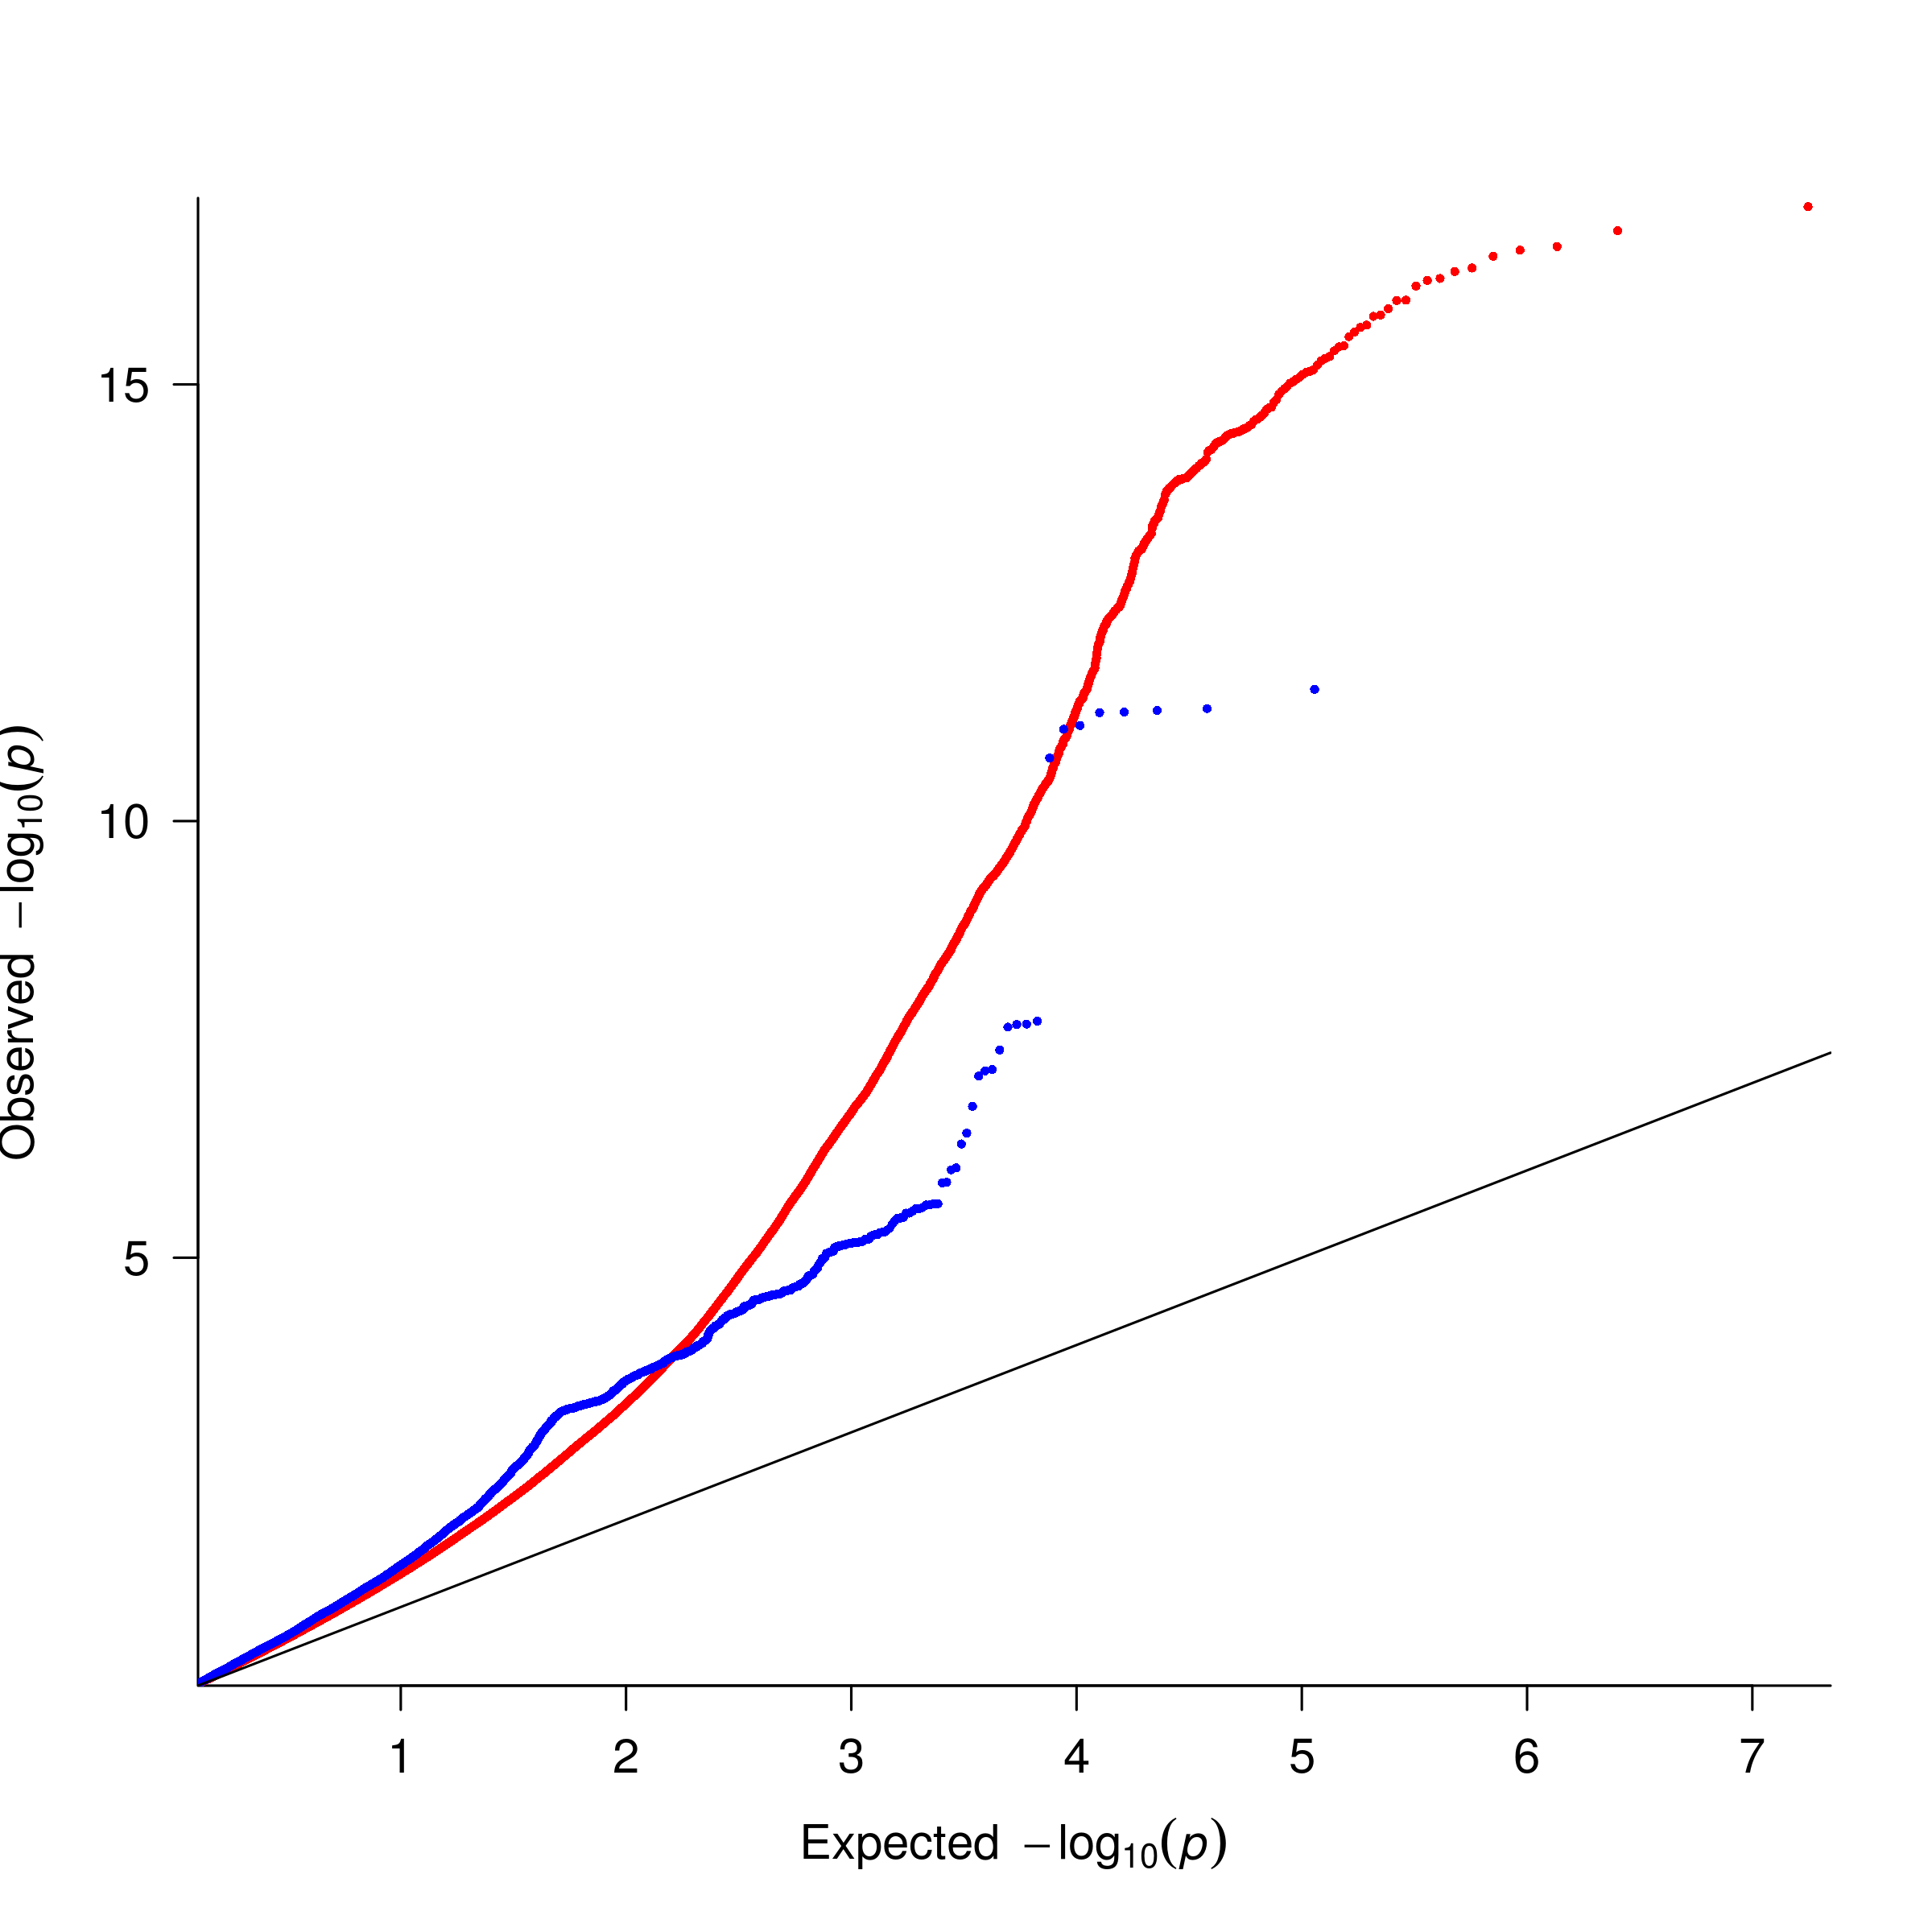
\includegraphics{figure/omega/NABA_CORE_MATRISOME.png}}
%		\label{fig:ecm}
%	}
%	\subfloat[MAPK Signaling]{
%		\scalebox{.4}{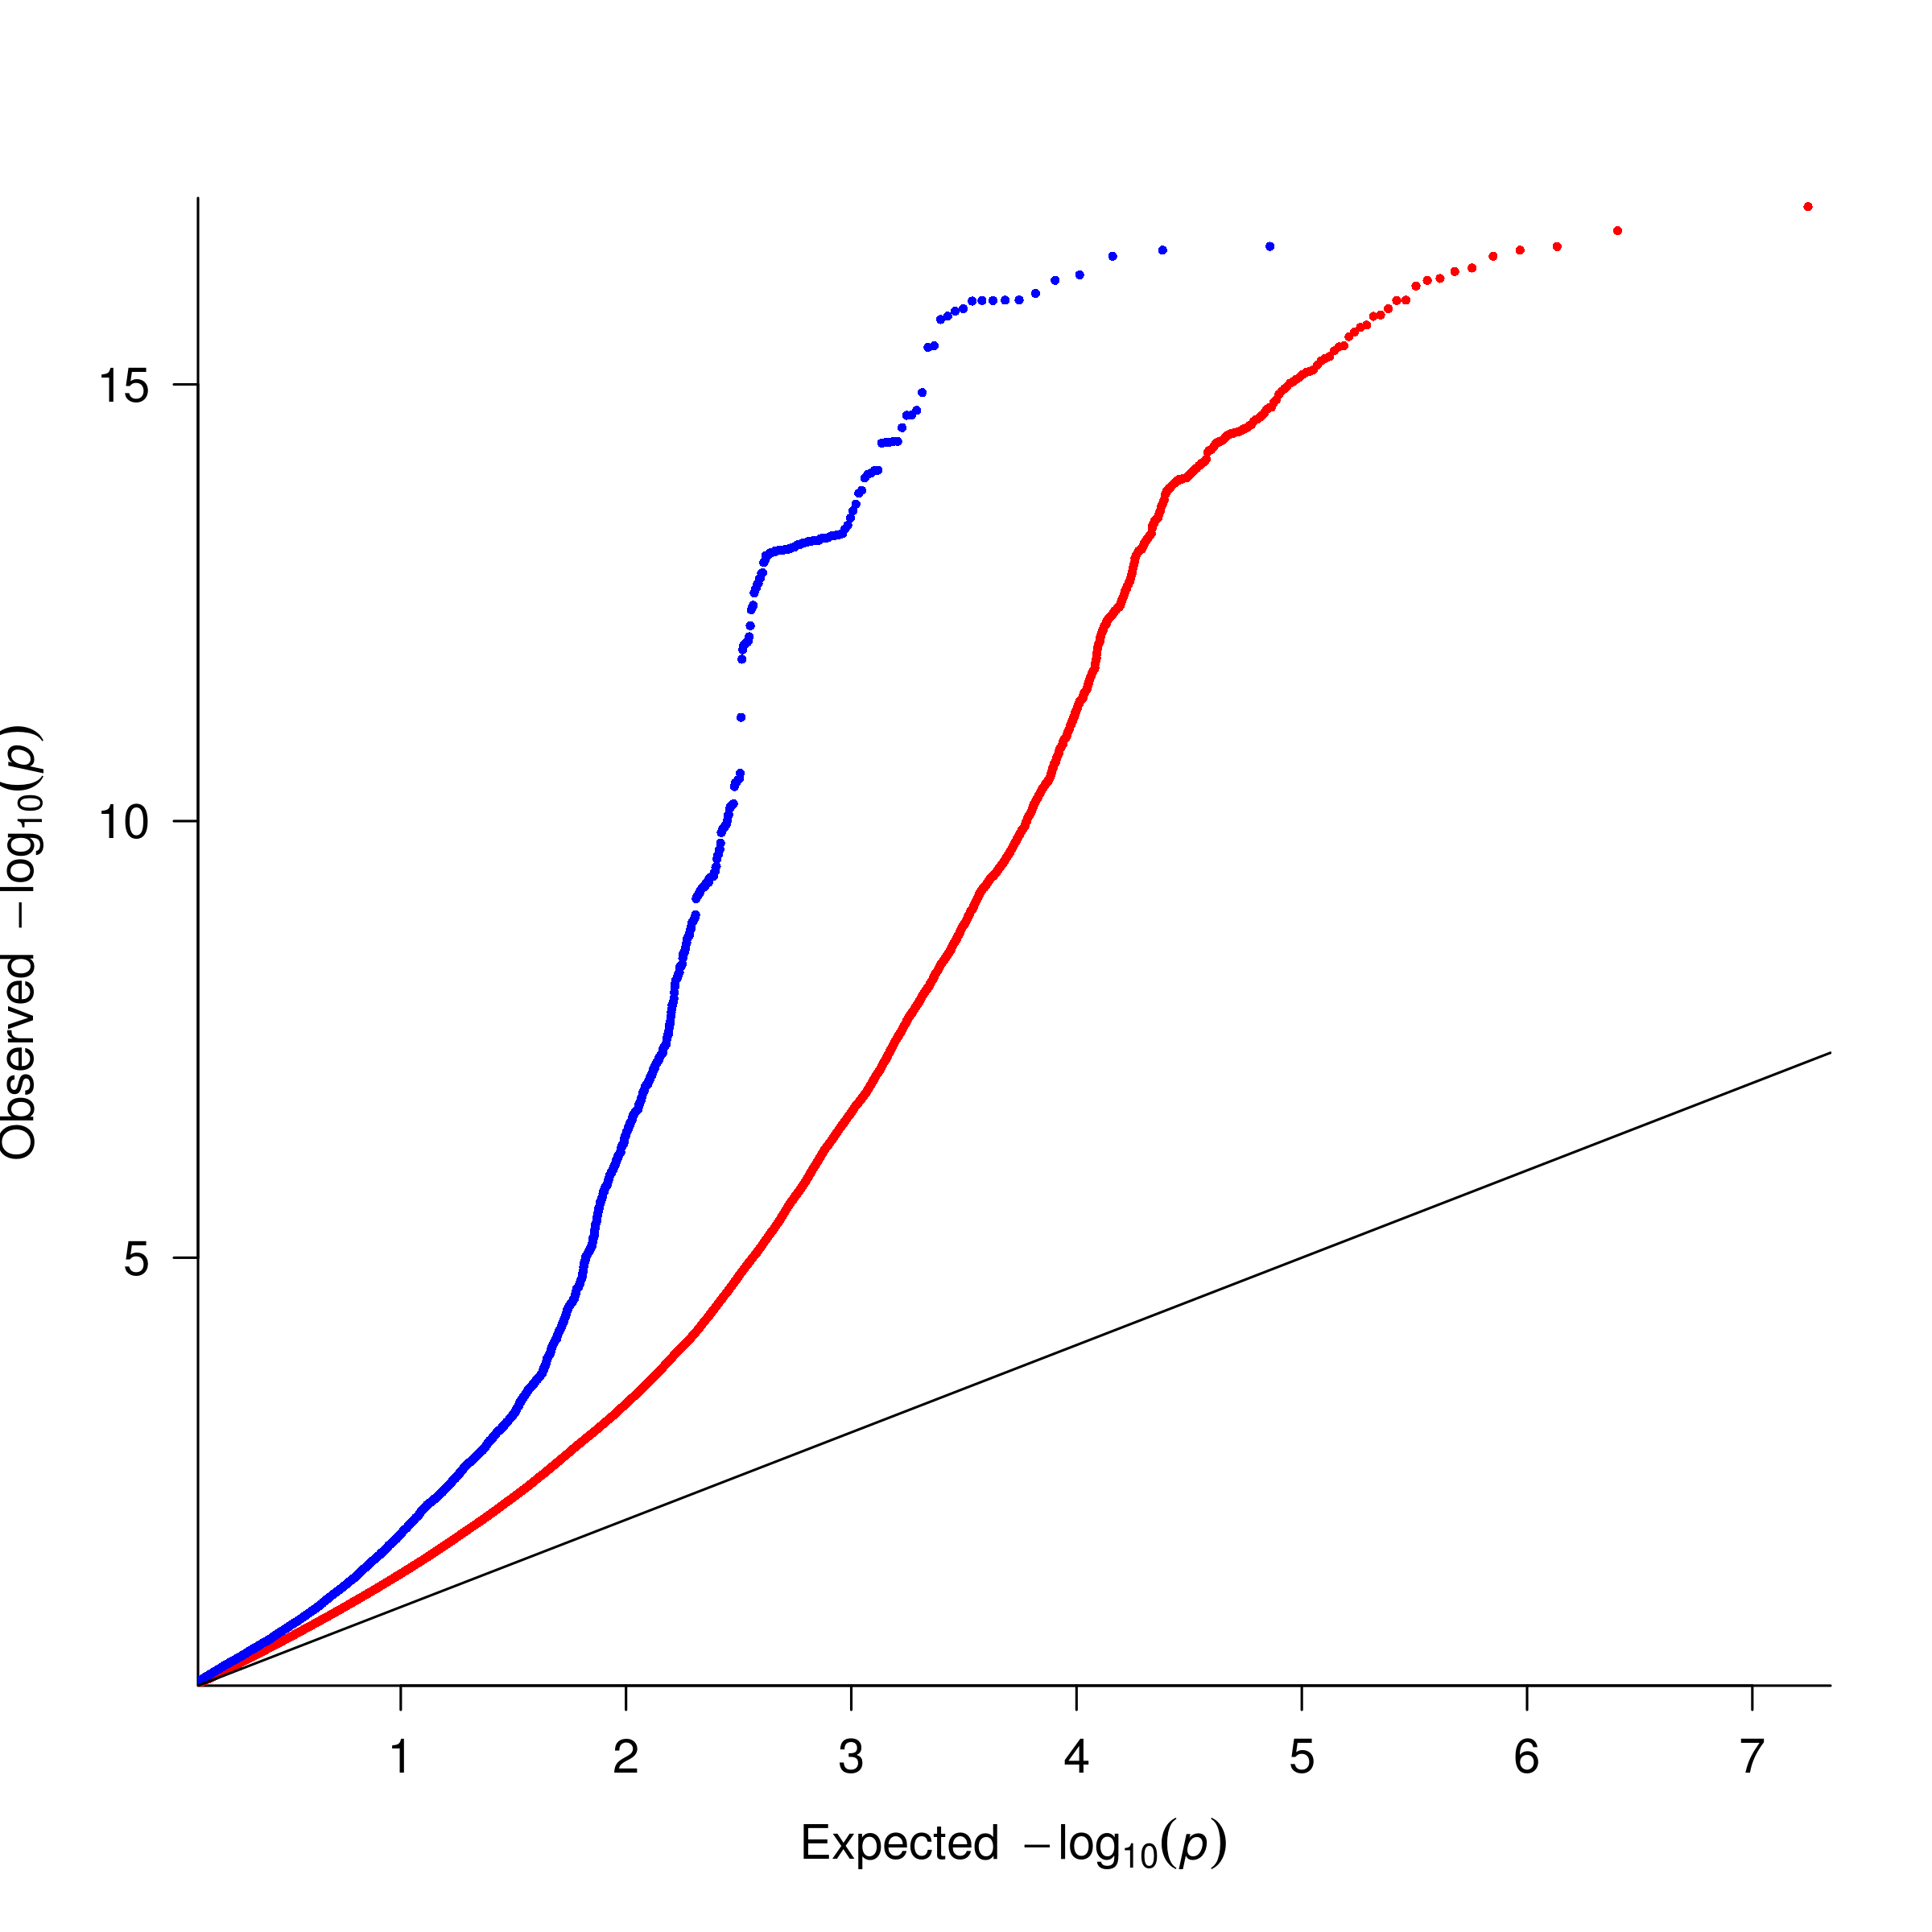
\includegraphics{figure/omega/KEGG_MAPK_SIGNALING_PATHWAY.png}}
%		\label{fig:mapk}
%	}\\
%	\subfloat[Neuronal System]{
%		\scalebox{.4}{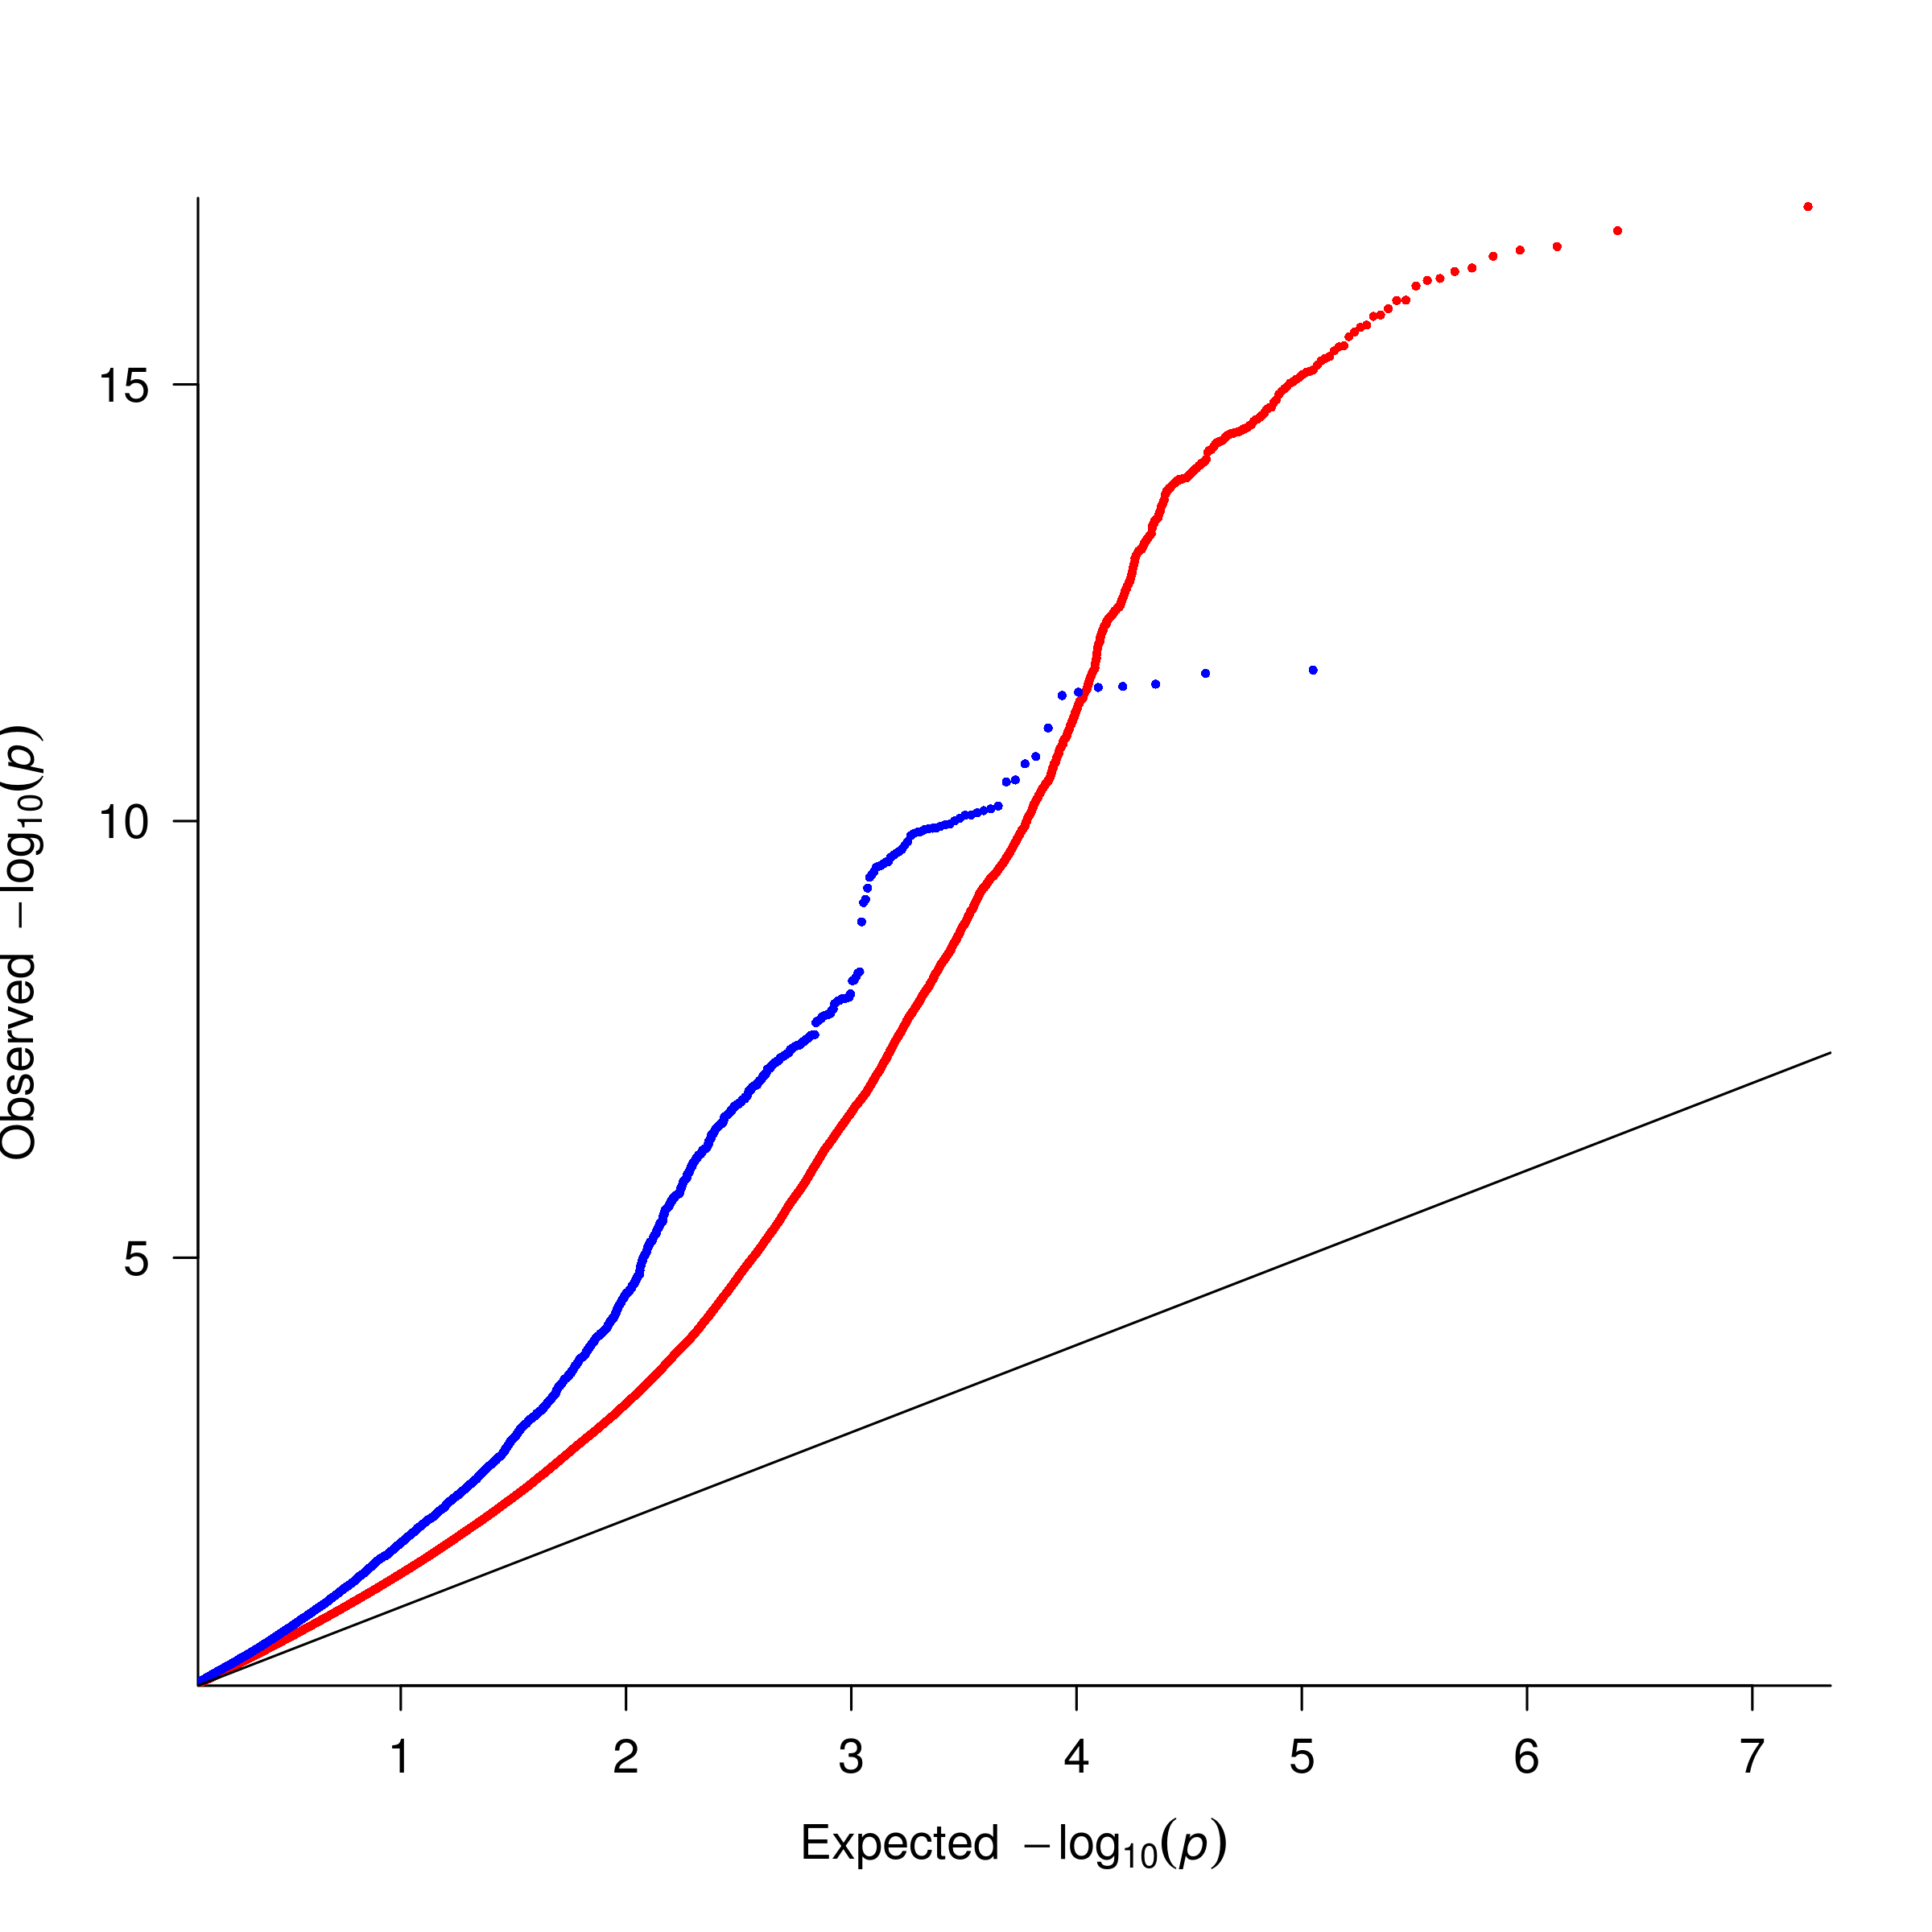
\includegraphics{figure/omega/REACTOME_NEURONAL_SYSTEM.png}}
%		\label{fig:neuronal}
%	}
%	\subfloat[Calcium Signaling]{
%		
%		\scalebox{.4}{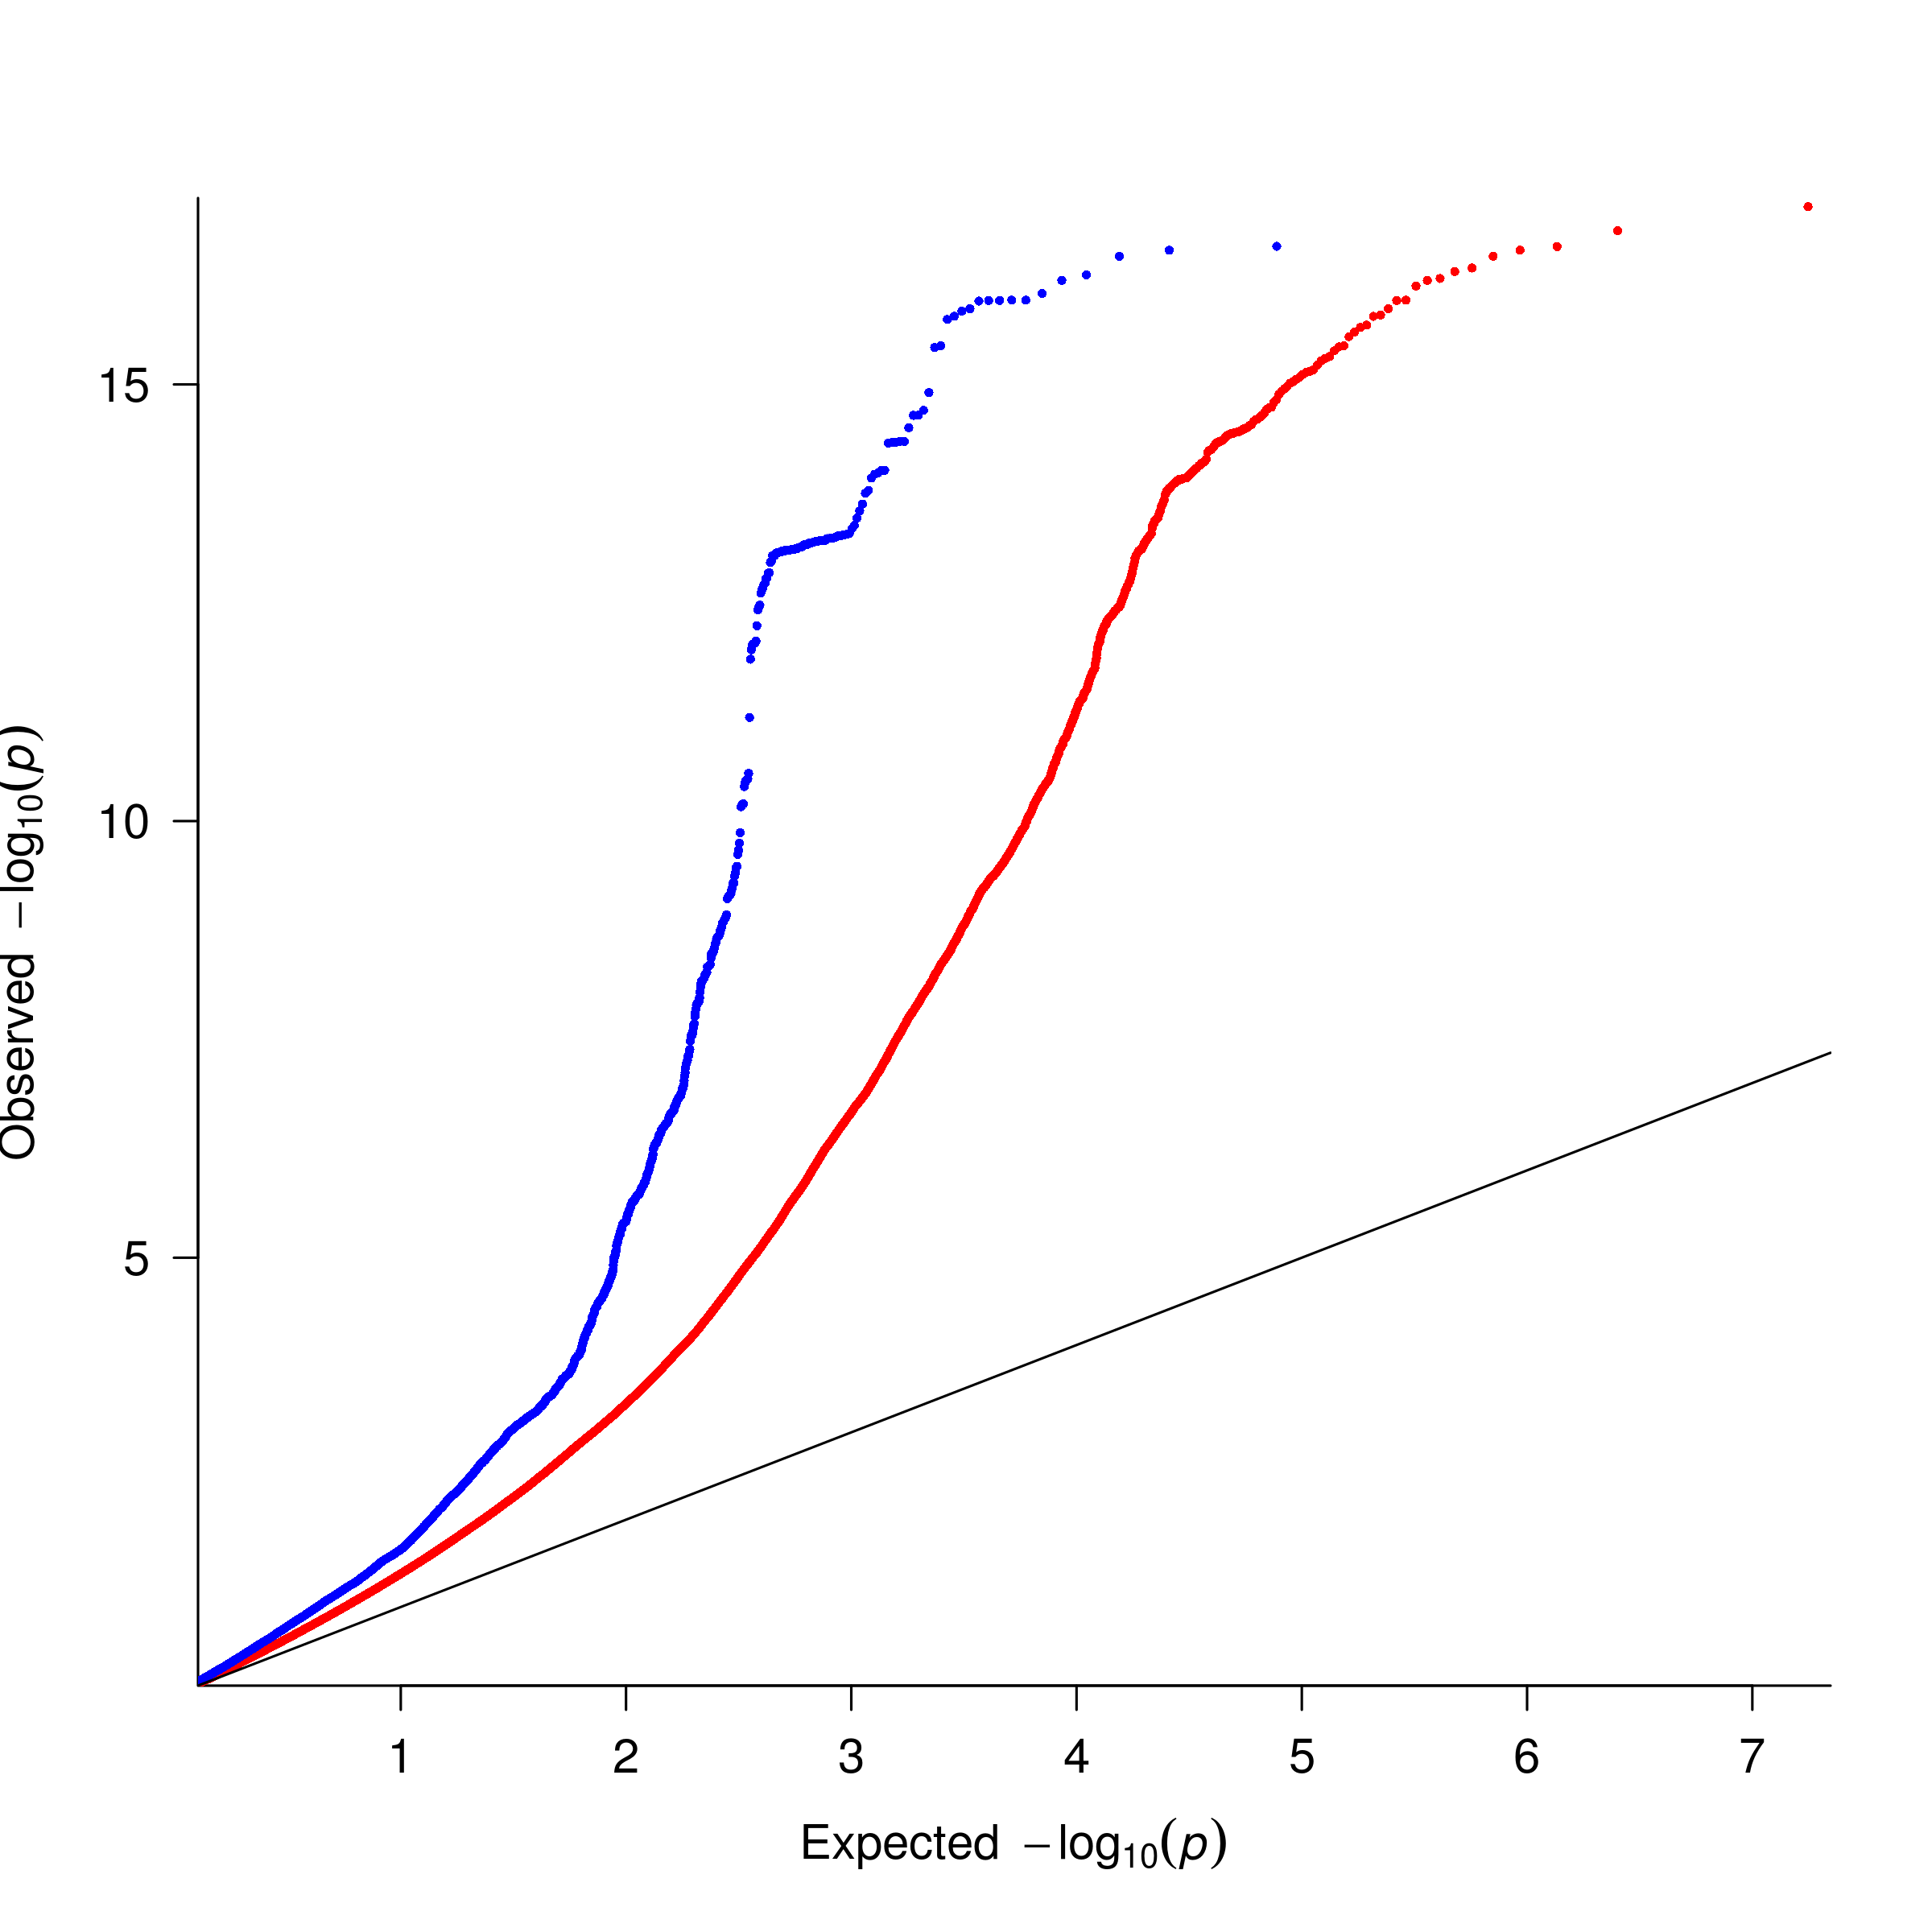
\includegraphics{figure/omega/KEGG_CALCIUM_SIGNALING_PATHWAY.png}}
%		\label{fig:calcium}
%	}
%	\caption[Comparing the QQ plots with PGC SNPs]
%	{Comparing the \gls{qqplot} with \gls{pgc} \glspl{SNP}.
%		\glspl{SNP} found within the pathways were colored in blue whereas the all the full set of \glspl{SNP} from the \gls{pgc} \gls{GWAS} was coded in red.
%		It is observed that for most of the pathways, there is a general inflation of summary statistics when compared to the full set, suggest that the significance was not driven by a single significant gene.
%		However, for the \gls{ecm} related pathway, only a small inflation was observed. 
%		This is therefore likely that the significance was driven by a small number of significant genes. 
%		} 
%	\label{fig:qqAll}
%\end{figure}
%
%The ``super pathway'' containing all the genes participating in the \gls{mia} related pathways were also found to be significant (\cref{tab:partitioning}) suggest that the differential gene expression in the cerebellum induced by early \gls{mia} events and the genetic variants might act upon similar pathways in the development of \glng{scz}.
%
%Interestingly, among the 4 pathways found to be significantly contributes to the \gls{SNP} heritability, only the pathway related to the assembly of core \gls{ecm} molecules such as the \gls{ecm} glycoproteins, were also found to be significantly affected by the n-3 \gls{pufa} rich diet in the \gls{polyic} exposed mouse. 
%Although the \gls{qqplot} suggest that a small number of genes might have driven the significance of this pathway, it is nonetheless an interesting candidate.
%
%Emerging evidences suggest that the \gls{ecm} abnormality might be associated with \glng{scz} \citep{Berretta2012}.
%The \gls{ecm} glycoprotein Reelin has been reported to have a decreased expression in the cerebellum of \glng{scz} patients \citep{Maloku2010} and were found to be accompanied by decreased expression of glutamic acid decarboxylase 67 \citep{Costa2001}.
%Studies also suggested that Reelin might have important role in corticogenesis and synaptic maturation and stabilization \citep{Berretta2012}.
%Moreover, another \gls{ecm} molecule, Semaphorin 3A has been reported to be increased in the cerebellum of subjects with \glng{scz} \citep{Eastwood2003}.
%The Semaphroin 3A protein was found to regulates axonal guidance and has a critical role in the  regulation of tangential migration of cortical GABAergic interneurons \citep{Zimmer2010}.
%It was also reported that the elevated Semaphorin 3A is associated with down-regulation of genes involved in synaptic formation and maintenance \citep{Eastwood2003}.
%Together, these evidence suggest that the \gls{ecm} molecules might have critical role in the development of \glng{scz}.
%
%It has been reported that the n-3 \gls{pufa} diet can modulate the \gls{mmp} \citep{Derosa2009,Kavazos2015} which can regulates the \gls{ecm} composition \citep{Stamenkovic2003}.
%Therefore it is possible that the n-3 \gls{pufa} diet has exerted its effect to the \gls{ecm} through \gls{mmp}.
%However, from the \gls{qqplot}, it was noted that only a modest inflation was observed (\cref{fig:ecm}).
%This suggest that the significance of the \gls{ecm} pathway might have been driven by a small number of significant genes.
%Due to difficulties in delineating the individual \glspl{SNP} effect, it is difficult for us to pin-point the ``driver'' genes of this pathway.
%Moreover, none of the \gls{ecm} genes were found to be differentially expressed in either of our condition, therefore we urge that further studies are required to understand how the n-3 \gls{pufa} direct interacts with the \gls{ecm} or the \gls{ecm} related genes and the effect of such interaction in \gls{mia} exposed individuals.
%
%Finally, it is important to note that the current study serves only as a hypothesis generation study and the sample size was modest. 
%We therefore like to use the current results to provide an estimation of sample size required for a replication study.
%By using Scotty \citep{Busby2013}, we have estimated that the replication study should contain at least 10 samples for each group in order for us to detect at least 80\% of genes has at least 80\% of the maximum power. 
%We have also demonstrated that the batch effect can have a big impact to the association (\cref{fig:batchLRT}), therefore one should always control for the batch effect whenever possible.
%Given the current resources, one of the preferred design for the follow up study are given in \cref{tab:bestdesign}.

\subsection{Limitations}
We first acknowledge that the sample size of the current study is moderate and might be underpowered.
This is reflected in the \glspl{qqplot} (\cref{fig:waldQQ}) where the observed p-values are generally smaller than expected.
An increased sample size is therefore required in order to obtain a larger detection power. 

Secondly, only the male brains were examined in the current study. 
The decision to direct experimental resources to males was made because there are evidences that the male fetus is more vulnerable to environmental exposures such as inflammation in prenatal life \citep{Bergeron2013,Lein2007}. 
An interesting follow up study would be to investigate the gender difference in response to \gls{mia} and dietary change.

Thirdly, although RNA Sequencing was performed, analysis on alternative splicing or de-novo transcript assembly were not performed.
It is because with the current sample size, there are insufficient information for de-novo transcript assembly to be performed. 
Most importantly, as we lack the resource for the functional analysis of de-novo transcripts, we cannot verify our findings, therefore the de-novo transcript assembly was not performed. 

On the other hand, to investigate possible alternative splicing events, analysis has to be performed on transcript level instead of gene level. 
This increases the possible candidates from 47,400 genes to 114,083 transcripts.
Therefore, a much larger detection power is required. 
Furthermore, the functional annotation of transcripts is difficult.
While there are a lot of information for the annotation of genes, information on functional difference between isoforms of the same gene are generally lacking. 
It is therefore difficult to understand the functional impact of the differential expression of different isoforms. 

In view of this, although alternative splicing and de-novo transcripts might play an important role in response to \gls{mia} or dietary changes, de-novo transcript assembly and alternative splicing analysis were not performed. 
Nevertheless, as RNA Sequencing was performed, de-novo transcript assembly and alternative splicing analysis can be performed when sufficient samples are collected in the future. 

Forthly, a high RNA expression level does not guarantee a high protein concentration \citep{Vogel2012}.
Post transcriptional, translational and degradation regulation can all affect the rates of protein production and turnover, therefore contributes to the determination of protein concentrations, at least as much as transcription itself \citep{Vogel2012}.
The RNA Sequencing thus only provide an approximation to the concentration of a particular protein in the samples.
Results from the RNA Sequencing study should serve as a candidates for further functional analysis protein assays in order to obtain a better understanding of the condition.

Finally, at the time of this thesis, \gls{rtpcr} and functional studies have not been performed to  validate our findings.
As RNA Sequencing does not provide any causal linkage between the phenotype and the differential expression functional studies must be carried out in order to validate the functional impact of the differential expression. 
Moreover, it is also important to validate the expression counts from RNA Sequencing using \gls{rtpcr}.
Currently, the \gls{rtpcr} on \textit{Sgk1} are in progress. 
Shall the results be validated, subsequent functional studies can be performed. 

\newpage
\section{Supplementary}
% Table generated by Excel2LaTeX from sheet 'Sheet1'
\begin{center}
	\begin{longtable}[H]{rrrrrr}
			\toprule
			Litter & Condition & Diet  & Cage  & Batch & Lane \\
			\midrule
			\endhead
			\hline
			\multicolumn{6}{c}{Continued}\\
			\bottomrule
			\endfoot
			\bottomrule
			\endlastfoot
			    1     & PolyIC & n-3 PUFA & 1     & 1     & 1 \\
			    1     & PolyIC & n-6 PUFA & 2     & 5     & 1 \\
			    2     & PolyIC & n-3 PUFA & 3     & 4     & 2 \\
			    2     & PolyIC & n-6 PUFA & 4     & 3     & 3 \\
			    3     & PolyIC & n-3 PUFA & 5     & 2     & 4 \\
			    3     & PolyIC & n-6 PUFA & 6     & 1     & 1 \\
			    4     & PolyIC & n-3 PUFA & 7     & 5     & 1 \\
			    4     & PolyIC & n-6 PUFA & 8     & 4     & 2 \\
			    5     & PolyIC & n-3 PUFA & 9     & 3     & 3 \\
			    5     & PolyIC & n-6 PUFA & 10    & 2     & 4 \\
			    6     & PolyIC & n-3 PUFA & 1     & 2     & 1 \\
			    6     & PolyIC & n-6 PUFA & 2     & 1     & 2 \\
			    7     & PolyIC & n-3 PUFA & 3     & 5     & 2 \\
			    7     & PolyIC & n-6 PUFA & 4     & 4     & 3 \\
			    8     & PolyIC & n-3 PUFA & 5     & 3     & 4 \\
			    8     & PolyIC & n-6 PUFA & 6     & 2     & 1 \\
			    9     & PolyIC & n-3 PUFA & 7     & 1     & 2 \\
			    9     & PolyIC & n-6 PUFA & 8     & 5     & 2 \\
			    10    & PolyIC & n-3 PUFA & 9     & 4     & 3 \\
			    10    & PolyIC & n-6 PUFA & 10    & 3     & 4 \\
			    11    & Saline & n-3 PUFA & 1     & 3     & 1 \\
			    11    & Saline & n-6 PUFA & 2     & 2     & 2 \\
			    12    & Saline & n-3 PUFA & 3     & 1     & 3 \\
			    12    & Saline & n-6 PUFA & 4     & 5     & 3 \\
			    13    & Saline & n-3 PUFA & 5     & 4     & 4 \\
			    13    & Saline & n-6 PUFA & 6     & 3     & 1 \\
			    14    & Saline & n-3 PUFA & 7     & 2     & 2 \\
			    14    & Saline & n-6 PUFA & 8     & 1     & 3 \\
			    15    & Saline & n-3 PUFA & 9     & 5     & 3 \\
			    15    & Saline & n-6 PUFA & 10    & 4     & 4 \\
			    16    & Saline & n-3 PUFA & 1     & 4     & 1 \\
			    16    & Saline & n-6 PUFA & 2     & 3     & 2 \\
			    17    & Saline & n-3 PUFA & 3     & 2     & 3 \\
			    17    & Saline & n-6 PUFA & 4     & 1     & 4 \\
			    18    & Saline & n-3 PUFA & 5     & 5     & 4 \\
			    18    & Saline & n-6 PUFA & 6     & 4     & 1 \\
			    19    & Saline & n-3 PUFA & 7     & 3     & 2 \\
			    19    & Saline & n-6 PUFA & 8     & 2     & 3 \\
			    20    & Saline & n-3 PUFA & 9     & 1     & 4 \\
			    20    & Saline & n-6 PUFA & 10    & 5     & 4 \\
			\bottomrule
		\caption[Design for Follow Up Study]{
			Design for follow up study.
			This design will allow one to balanced out litter effect, cage effect, batch effect and lane effects such that the confounding effects were minimized.
			One can also include the \gls{ercc} spike in control to serves as an internal standard for additional level of control \citep{Jiang2011a}.
			}
		\label{tab:bestdesign}%
	\end{longtable}%ssss
\end{center}
% End up it is very easy, all you have to do is to first sort the table with the previous condition then e.g. Cage, then repeat the number of condition e.g. 1,2,1,2,1,2 until the end. Keep doing that and you will have a best mixed model